\documentclass[11pt,]{article}
\usepackage{lmodern}
\usepackage{amssymb,amsmath}
\usepackage{ifxetex,ifluatex}
\usepackage{fixltx2e} % provides \textsubscript
\ifnum 0\ifxetex 1\fi\ifluatex 1\fi=0 % if pdftex
  \usepackage[T1]{fontenc}
  \usepackage[utf8]{inputenc}
\else % if luatex or xelatex
  \ifxetex
    \usepackage{mathspec}
  \else
    \usepackage{fontspec}
  \fi
  \defaultfontfeatures{Ligatures=TeX,Scale=MatchLowercase}
\fi
% use upquote if available, for straight quotes in verbatim environments
\IfFileExists{upquote.sty}{\usepackage{upquote}}{}
% use microtype if available
\IfFileExists{microtype.sty}{%
\usepackage{microtype}
\UseMicrotypeSet[protrusion]{basicmath} % disable protrusion for tt fonts
}{}
\usepackage[margin=1in]{geometry}
\usepackage{hyperref}
\hypersetup{unicode=true,
            pdftitle={Appendix S3. Steps to recreate figures from main text.},
            pdfborder={0 0 0},
            breaklinks=true}
\urlstyle{same}  % don't use monospace font for urls
\usepackage{color}
\usepackage{fancyvrb}
\newcommand{\VerbBar}{|}
\newcommand{\VERB}{\Verb[commandchars=\\\{\}]}
\DefineVerbatimEnvironment{Highlighting}{Verbatim}{commandchars=\\\{\}}
% Add ',fontsize=\small' for more characters per line
\newenvironment{Shaded}{}{}
\newcommand{\AlertTok}[1]{\textcolor[rgb]{1.00,0.00,0.00}{#1}}
\newcommand{\AnnotationTok}[1]{\textcolor[rgb]{0.00,0.50,0.00}{#1}}
\newcommand{\AttributeTok}[1]{#1}
\newcommand{\BaseNTok}[1]{#1}
\newcommand{\BuiltInTok}[1]{#1}
\newcommand{\CharTok}[1]{\textcolor[rgb]{0.00,0.50,0.50}{#1}}
\newcommand{\CommentTok}[1]{\textcolor[rgb]{0.00,0.50,0.00}{#1}}
\newcommand{\CommentVarTok}[1]{\textcolor[rgb]{0.00,0.50,0.00}{#1}}
\newcommand{\ConstantTok}[1]{#1}
\newcommand{\ControlFlowTok}[1]{\textcolor[rgb]{0.00,0.00,1.00}{#1}}
\newcommand{\DataTypeTok}[1]{#1}
\newcommand{\DecValTok}[1]{#1}
\newcommand{\DocumentationTok}[1]{\textcolor[rgb]{0.00,0.50,0.00}{#1}}
\newcommand{\ErrorTok}[1]{\textcolor[rgb]{1.00,0.00,0.00}{\textbf{#1}}}
\newcommand{\ExtensionTok}[1]{#1}
\newcommand{\FloatTok}[1]{#1}
\newcommand{\FunctionTok}[1]{#1}
\newcommand{\ImportTok}[1]{#1}
\newcommand{\InformationTok}[1]{\textcolor[rgb]{0.00,0.50,0.00}{#1}}
\newcommand{\KeywordTok}[1]{\textcolor[rgb]{0.00,0.00,1.00}{#1}}
\newcommand{\NormalTok}[1]{#1}
\newcommand{\OperatorTok}[1]{#1}
\newcommand{\OtherTok}[1]{\textcolor[rgb]{1.00,0.25,0.00}{#1}}
\newcommand{\PreprocessorTok}[1]{\textcolor[rgb]{1.00,0.25,0.00}{#1}}
\newcommand{\RegionMarkerTok}[1]{#1}
\newcommand{\SpecialCharTok}[1]{\textcolor[rgb]{0.00,0.50,0.50}{#1}}
\newcommand{\SpecialStringTok}[1]{\textcolor[rgb]{0.00,0.50,0.50}{#1}}
\newcommand{\StringTok}[1]{\textcolor[rgb]{0.00,0.50,0.50}{#1}}
\newcommand{\VariableTok}[1]{#1}
\newcommand{\VerbatimStringTok}[1]{\textcolor[rgb]{0.00,0.50,0.50}{#1}}
\newcommand{\WarningTok}[1]{\textcolor[rgb]{0.00,0.50,0.00}{\textbf{#1}}}
\usepackage{graphicx,grffile}
\makeatletter
\def\maxwidth{\ifdim\Gin@nat@width>\linewidth\linewidth\else\Gin@nat@width\fi}
\def\maxheight{\ifdim\Gin@nat@height>\textheight\textheight\else\Gin@nat@height\fi}
\makeatother
% Scale images if necessary, so that they will not overflow the page
% margins by default, and it is still possible to overwrite the defaults
% using explicit options in \includegraphics[width, height, ...]{}
\setkeys{Gin}{width=\maxwidth,height=\maxheight,keepaspectratio}
\IfFileExists{parskip.sty}{%
\usepackage{parskip}
}{% else
\setlength{\parindent}{0pt}
\setlength{\parskip}{6pt plus 2pt minus 1pt}
}
\setlength{\emergencystretch}{3em}  % prevent overfull lines
\providecommand{\tightlist}{%
  \setlength{\itemsep}{0pt}\setlength{\parskip}{0pt}}
\setcounter{secnumdepth}{5}
% Redefines (sub)paragraphs to behave more like sections
\ifx\paragraph\undefined\else
\let\oldparagraph\paragraph
\renewcommand{\paragraph}[1]{\oldparagraph{#1}\mbox{}}
\fi
\ifx\subparagraph\undefined\else
\let\oldsubparagraph\subparagraph
\renewcommand{\subparagraph}[1]{\oldsubparagraph{#1}\mbox{}}
\fi

%%% Use protect on footnotes to avoid problems with footnotes in titles
\let\rmarkdownfootnote\footnote%
\def\footnote{\protect\rmarkdownfootnote}

%%% Change title format to be more compact
\usepackage{titling}

% Create subtitle command for use in maketitle
\providecommand{\subtitle}[1]{
  \posttitle{
    \begin{center}\large#1\end{center}
    }
}

\setlength{\droptitle}{-2em}

  \title{Appendix S3. Steps to recreate figures from main text.}
    \pretitle{\vspace{\droptitle}\centering\huge}
  \posttitle{\par}
  \subtitle{Supporting information for Scheuerell et al.}
  \author{}
    \preauthor{}\postauthor{}
    \date{}
    \predate{}\postdate{}
  

\begin{document}
\maketitle

{
\setcounter{tocdepth}{3}
\tableofcontents
}
\vspace{0.2in}

This is version 0.19.07.08.

\hypertarget{background}{%
\section{Background}\label{background}}

This appendix shows how to recreate the figures in the main text based
on the results from the best of the fitted models.

All analyses require the \href{https://cran.r-project.org/}{R software}
(v3.4.3 or later), as well as a few packages that are not included with
the base installation of R.

\begin{Shaded}
\begin{Highlighting}[]
\ControlFlowTok{if}\NormalTok{(}\OperatorTok{!}\KeywordTok{require}\NormalTok{(}\StringTok{"readr"}\NormalTok{)) \{}
  \KeywordTok{install.packages}\NormalTok{(}\StringTok{"readr"}\NormalTok{)}
  \KeywordTok{library}\NormalTok{(}\StringTok{"readr"}\NormalTok{)}
\NormalTok{\}}
\ControlFlowTok{if}\NormalTok{(}\OperatorTok{!}\KeywordTok{require}\NormalTok{(}\StringTok{"captioner"}\NormalTok{)) \{}
\NormalTok{  devtools}\OperatorTok{::}\KeywordTok{install_github}\NormalTok{(}\StringTok{"adletaw/captioner"}\NormalTok{)}
  \KeywordTok{library}\NormalTok{(}\StringTok{"captioner"}\NormalTok{)}
\NormalTok{\}}
\NormalTok{fig_cap <-}\StringTok{ }\KeywordTok{captioner}\NormalTok{(}\DataTypeTok{suffix =} \StringTok{"."}\NormalTok{)}
\ControlFlowTok{if}\NormalTok{(}\OperatorTok{!}\KeywordTok{require}\NormalTok{(}\StringTok{"coda"}\NormalTok{)) \{}
  \KeywordTok{install.packages}\NormalTok{(}\StringTok{"coda"}\NormalTok{)}
  \KeywordTok{library}\NormalTok{(}\StringTok{"coda"}\NormalTok{)}
\NormalTok{\}}
\ControlFlowTok{if}\NormalTok{(}\OperatorTok{!}\KeywordTok{require}\NormalTok{(}\StringTok{"here"}\NormalTok{)) \{}
  \KeywordTok{install.packages}\NormalTok{(}\StringTok{"here"}\NormalTok{)}
  \KeywordTok{library}\NormalTok{(}\StringTok{"here"}\NormalTok{)}
\NormalTok{\}}
\ControlFlowTok{if}\NormalTok{(}\OperatorTok{!}\KeywordTok{require}\NormalTok{(}\StringTok{"gsl"}\NormalTok{)) \{}
  \KeywordTok{install.packages}\NormalTok{(}\StringTok{"gsl"}\NormalTok{)}
  \KeywordTok{library}\NormalTok{(}\StringTok{"gsl"}\NormalTok{)}
\NormalTok{\}}
\CommentTok{## set directory locations}
\NormalTok{datadir <-}\StringTok{ }\KeywordTok{here}\NormalTok{(}\StringTok{"data"}\NormalTok{)}
\NormalTok{analdir <-}\StringTok{ }\KeywordTok{here}\NormalTok{(}\StringTok{"analysis"}\NormalTok{)}
\NormalTok{savedir <-}\StringTok{ }\KeywordTok{here}\NormalTok{(}\StringTok{"analysis/cache"}\NormalTok{)}
\end{Highlighting}
\end{Shaded}

We also need a couple of helper functions.

\begin{Shaded}
\begin{Highlighting}[]
\CommentTok{## better round}
\NormalTok{Re2prec <-}\StringTok{ }\ControlFlowTok{function}\NormalTok{(x, }\DataTypeTok{map =} \StringTok{"round"}\NormalTok{, }\DataTypeTok{prec =} \DecValTok{1}\NormalTok{) \{}
  \CommentTok{## 'map' can be "round", "floor", or "ceiling"}
  \CommentTok{## 'prec' is nearest value}
  \CommentTok{## (eg, 0.1 is to nearest tenth; 1 is to nearest integer)}
  \ControlFlowTok{if}\NormalTok{(prec }\OperatorTok{<=}\StringTok{ }\DecValTok{0}\NormalTok{) \{}
    \KeywordTok{stop}\NormalTok{(}\StringTok{"}\CharTok{\textbackslash{}"}\StringTok{prec}\CharTok{\textbackslash{}"}\StringTok{ cannot be less than or equal to 0"}\NormalTok{)}
\NormalTok{  \}}
  \KeywordTok{do.call}\NormalTok{(map, }\KeywordTok{list}\NormalTok{(x }\OperatorTok{/}\StringTok{ }\NormalTok{prec)) }\OperatorTok{*}\StringTok{ }\NormalTok{prec}
\NormalTok{\}}
\end{Highlighting}
\end{Shaded}

\hypertarget{load-the-information}{%
\section{Load the information}\label{load-the-information}}

Here we load in the model fits, covariates, and harvest data.

\begin{Shaded}
\begin{Highlighting}[]
\NormalTok{best_fit <-}\StringTok{ }\KeywordTok{readRDS}\NormalTok{(}\KeywordTok{file.path}\NormalTok{(savedir, }\StringTok{"fit_bh_cov.rds"}\NormalTok{))}
\end{Highlighting}
\end{Shaded}

\begin{Shaded}
\begin{Highlighting}[]
\CommentTok{## covariate(s)}
\NormalTok{dat_cvrs <-}\StringTok{ }\KeywordTok{read_csv}\NormalTok{(}\KeywordTok{file.path}\NormalTok{(datadir, }\StringTok{"skagit_sthd_covars.csv"}\NormalTok{))}
\CommentTok{## total number of covariates}
\NormalTok{n_cov <-}\StringTok{ }\KeywordTok{dim}\NormalTok{(dat_cvrs)[}\DecValTok{2}\NormalTok{] }\OperatorTok{-}\StringTok{ }\DecValTok{1}
\end{Highlighting}
\end{Shaded}

\begin{Shaded}
\begin{Highlighting}[]
\CommentTok{## escapement}
\NormalTok{dat_esc <-}\StringTok{ }\KeywordTok{read_csv}\NormalTok{(}\KeywordTok{file.path}\NormalTok{(datadir, }\StringTok{"skagit_sthd_esc.csv"}\NormalTok{))}
\CommentTok{## log of escapement}
\NormalTok{ln_dat_esc <-}\StringTok{ }\KeywordTok{c}\NormalTok{(}\KeywordTok{log}\NormalTok{(dat_esc}\OperatorTok{$}\NormalTok{escapement), }\KeywordTok{rep}\NormalTok{(}\OtherTok{NA}\NormalTok{, n_fore))}
\end{Highlighting}
\end{Shaded}

\begin{Shaded}
\begin{Highlighting}[]
\CommentTok{## harvest}
\NormalTok{dat_harv <-}\StringTok{ }\KeywordTok{read_csv}\NormalTok{(}\KeywordTok{file.path}\NormalTok{(datadir, }\StringTok{"skagit_sthd_catch.csv"}\NormalTok{))}
\CommentTok{## drop year col & first age_max rows}
\NormalTok{dat_harv <-}\StringTok{ }\KeywordTok{c}\NormalTok{(dat_harv}\OperatorTok{$}\NormalTok{catch, }\KeywordTok{rep}\NormalTok{(}\DecValTok{0}\NormalTok{, n_fore))}
\end{Highlighting}
\end{Shaded}

\hypertarget{model-forms}{%
\section{Model forms}\label{model-forms}}

Here are schematics of the deterministic forms of process models used in
the analyses.

\begin{Shaded}
\begin{Highlighting}[]
\CommentTok{## params}
\CommentTok{## Ricker}
\NormalTok{ra <-}\StringTok{ }\DecValTok{3}
\NormalTok{rb <-}\StringTok{ }\FloatTok{1.2e-4}
\CommentTok{## B-H}
\NormalTok{ba <-}\StringTok{ }\DecValTok{3}
\NormalTok{bb <-}\StringTok{ }\DecValTok{3}\OperatorTok{/}\FloatTok{1.4e4}

\CommentTok{## ref pts}
\CommentTok{## Ricker}
\NormalTok{rmr <-}\StringTok{ }\NormalTok{ra}\OperatorTok{/}\NormalTok{rb}\OperatorTok{*}\KeywordTok{exp}\NormalTok{(}\OperatorTok{-}\DecValTok{1}\NormalTok{)}
\NormalTok{rsy <-}\StringTok{ }\NormalTok{(}\DecValTok{1} \OperatorTok{-}\StringTok{ }\KeywordTok{lambert_W0}\NormalTok{(}\KeywordTok{exp}\NormalTok{(}\DecValTok{1}\NormalTok{)}\OperatorTok{/}\NormalTok{ra)) }\OperatorTok{/}\StringTok{ }\NormalTok{rb}
\NormalTok{ruy <-}\StringTok{ }\DecValTok{1} \OperatorTok{-}\StringTok{ }\KeywordTok{lambert_W0}\NormalTok{(}\KeywordTok{exp}\NormalTok{(}\DecValTok{1}\NormalTok{)}\OperatorTok{/}\NormalTok{ra)}
\CommentTok{## B-H}
\NormalTok{bmr <-}\StringTok{ }\NormalTok{ba}\OperatorTok{/}\NormalTok{bb}
\NormalTok{bsy <-}\StringTok{ }\NormalTok{(ba}\OperatorTok{/}\NormalTok{bb)}\OperatorTok{*}\KeywordTok{sqrt}\NormalTok{(}\DecValTok{1}\OperatorTok{/}\NormalTok{ba)}\OperatorTok{-}\NormalTok{(}\DecValTok{1}\OperatorTok{/}\NormalTok{bb)}
\NormalTok{bsy <-}\StringTok{ }\NormalTok{(}\KeywordTok{sqrt}\NormalTok{(ba)}\OperatorTok{-}\DecValTok{1}\NormalTok{)}\OperatorTok{/}\NormalTok{bb}
\NormalTok{buy <-}\StringTok{ }\DecValTok{1} \OperatorTok{-}\StringTok{ }\KeywordTok{sqrt}\NormalTok{(}\DecValTok{1}\OperatorTok{/}\NormalTok{ba)}

\CommentTok{## S-R curves}
\CommentTok{## spawners}
\NormalTok{ss <-}\StringTok{ }\KeywordTok{seq}\NormalTok{(}\DecValTok{0}\NormalTok{,}\FloatTok{1.2e4}\NormalTok{,}\DecValTok{10}\NormalTok{)}
\CommentTok{## Ricker}
\NormalTok{rr <-}\StringTok{ }\NormalTok{ra}\OperatorTok{*}\NormalTok{ss}\OperatorTok{/}\KeywordTok{exp}\NormalTok{(rb}\OperatorTok{*}\NormalTok{ss)}
\CommentTok{## B-H}
\NormalTok{br <-}\StringTok{ }\NormalTok{ba}\OperatorTok{*}\NormalTok{ss}\OperatorTok{/}\NormalTok{(}\DecValTok{1} \OperatorTok{+}\StringTok{ }\NormalTok{bb}\OperatorTok{*}\NormalTok{ss)}

\CommentTok{## plots}

\KeywordTok{layout}\NormalTok{(}\KeywordTok{matrix}\NormalTok{(}\KeywordTok{c}\NormalTok{(}\DecValTok{1}\NormalTok{,}\DecValTok{0}\NormalTok{,}\DecValTok{2}\NormalTok{),}\DecValTok{3}\NormalTok{,}\DecValTok{1}\NormalTok{), }\DataTypeTok{heights=}\KeywordTok{lcm}\NormalTok{(}\KeywordTok{c}\NormalTok{(}\DecValTok{3}\NormalTok{,}\FloatTok{0.3}\NormalTok{,}\DecValTok{3}\NormalTok{)}\OperatorTok{*}\FloatTok{2.54}\NormalTok{), }\DataTypeTok{widths=}\KeywordTok{lcm}\NormalTok{(}\DecValTok{3}\OperatorTok{*}\FloatTok{2.54}\NormalTok{))}
\KeywordTok{par}\NormalTok{(}\DataTypeTok{mai=}\KeywordTok{c}\NormalTok{(}\FloatTok{0.4}\NormalTok{,}\FloatTok{0.4}\NormalTok{,}\FloatTok{0.2}\NormalTok{,}\FloatTok{0.2}\NormalTok{), }\DataTypeTok{omi=}\KeywordTok{c}\NormalTok{(}\DecValTok{0}\NormalTok{,}\DecValTok{0}\NormalTok{,}\DecValTok{0}\NormalTok{,}\FloatTok{0.25}\NormalTok{))}

\CommentTok{## Ricker}
\KeywordTok{plot}\NormalTok{(ss, rr, }\DataTypeTok{type=}\StringTok{"n"}\NormalTok{, }\DataTypeTok{xlim=}\KeywordTok{range}\NormalTok{(ss), }\DataTypeTok{ylim=}\KeywordTok{range}\NormalTok{(ss), }\DataTypeTok{xaxs=}\StringTok{"i"}\NormalTok{, }\DataTypeTok{yaxs=}\StringTok{"i"}\NormalTok{,}
     \DataTypeTok{xlab=}\StringTok{""}\NormalTok{, }\DataTypeTok{ylab=}\StringTok{""}\NormalTok{, }\DataTypeTok{xaxt=}\StringTok{"n"}\NormalTok{, }\DataTypeTok{yaxt=}\StringTok{"n"}\NormalTok{, }\DataTypeTok{bty=}\StringTok{"L"}\NormalTok{)}
\KeywordTok{mtext}\NormalTok{(}\KeywordTok{expression}\NormalTok{(}\KeywordTok{italic}\NormalTok{(S[t])), }\DecValTok{1}\NormalTok{, }\DataTypeTok{line=}\DecValTok{1}\NormalTok{, }\DataTypeTok{cex=}\FloatTok{1.1}\NormalTok{, }\DataTypeTok{at=}\KeywordTok{max}\NormalTok{(ss))}
\KeywordTok{mtext}\NormalTok{(}\KeywordTok{expression}\NormalTok{(}\KeywordTok{italic}\NormalTok{(R[t])), }\DecValTok{2}\NormalTok{, }\DataTypeTok{line=}\FloatTok{0.5}\NormalTok{, }\DataTypeTok{cex=}\FloatTok{1.1}\NormalTok{, }\DataTypeTok{at=}\KeywordTok{max}\NormalTok{(ss), }\DataTypeTok{las=}\DecValTok{1}\NormalTok{)}
\NormalTok{rttl <-}\StringTok{ "(a) Ricker"}
\KeywordTok{text}\NormalTok{(}\DecValTok{400}\NormalTok{, }\KeywordTok{max}\NormalTok{(ss), rttl, }\DataTypeTok{cex=}\FloatTok{1.1}\NormalTok{, }\DataTypeTok{adj=}\KeywordTok{c}\NormalTok{(}\DecValTok{0}\NormalTok{,}\DecValTok{1}\NormalTok{), }\DataTypeTok{xpd=}\OtherTok{NA}\NormalTok{)}
\CommentTok{## 1:1}
\KeywordTok{abline}\NormalTok{(}\DataTypeTok{a=}\DecValTok{0}\NormalTok{, }\DataTypeTok{b=}\DecValTok{1}\NormalTok{, }\DataTypeTok{col=}\StringTok{"gray"}\NormalTok{)}
\CommentTok{#text(1.2e4, 1.2e4, "1:1", adj=c(1,0))}
\CommentTok{## R-S}
\KeywordTok{lines}\NormalTok{(ss, rr, }\DataTypeTok{lwd=}\DecValTok{2}\NormalTok{)}
\NormalTok{rmod <-}\StringTok{ }\KeywordTok{expression}\NormalTok{(}\KeywordTok{frac}\NormalTok{(}\KeywordTok{italic}\NormalTok{(alpha }\OperatorTok{*}\StringTok{ }\NormalTok{S[t]),}\KeywordTok{italic}\NormalTok{(e}\OperatorTok{^}\NormalTok{\{beta }\OperatorTok{*}\StringTok{ }\NormalTok{S[t]\})))}
\KeywordTok{text}\NormalTok{(}\DecValTok{12300}\NormalTok{, ra}\OperatorTok{*}\KeywordTok{max}\NormalTok{(ss)}\OperatorTok{/}\KeywordTok{exp}\NormalTok{(rb}\OperatorTok{*}\KeywordTok{max}\NormalTok{(ss)), rmod, }\DataTypeTok{adj=}\KeywordTok{c}\NormalTok{(}\DecValTok{0}\NormalTok{,}\FloatTok{0.5}\NormalTok{), }\DataTypeTok{xpd=}\OtherTok{NA}\NormalTok{)}
\CommentTok{## alpha}
\KeywordTok{segments}\NormalTok{(}\DecValTok{0}\NormalTok{, }\DecValTok{0}\NormalTok{, }\DecValTok{1900}\NormalTok{, ra}\OperatorTok{*}\DecValTok{1900}\NormalTok{, }\DataTypeTok{lty=}\StringTok{"dashed"}\NormalTok{)}
\KeywordTok{text}\NormalTok{(}\DecValTok{2000}\NormalTok{, ra}\OperatorTok{*}\DecValTok{2000}\NormalTok{, }\KeywordTok{expression}\NormalTok{(alpha), }\DataTypeTok{adj=}\KeywordTok{c}\NormalTok{(}\FloatTok{0.5}\NormalTok{,}\FloatTok{0.5}\NormalTok{))}
\CommentTok{## MSY}
\KeywordTok{segments}\NormalTok{(rsy,}\DecValTok{0}\NormalTok{,rsy,ra}\OperatorTok{*}\NormalTok{rsy}\OperatorTok{/}\KeywordTok{exp}\NormalTok{(rb}\OperatorTok{*}\NormalTok{rsy), }\DataTypeTok{lty=}\StringTok{"dashed"}\NormalTok{)}
\KeywordTok{text}\NormalTok{(rsy, }\DecValTok{0}\NormalTok{, }\KeywordTok{expression}\NormalTok{(}\KeywordTok{frac}\NormalTok{(}\DecValTok{1}\OperatorTok{-}\KeywordTok{italic}\NormalTok{(W)}\OperatorTok{~}\KeywordTok{bgroup}\NormalTok{(}\StringTok{"("}\NormalTok{,}\KeywordTok{frac}\NormalTok{(}\KeywordTok{italic}\NormalTok{(e),alpha),}\StringTok{")"}\NormalTok{),beta)), }\DataTypeTok{adj=}\KeywordTok{c}\NormalTok{(}\FloatTok{0.5}\NormalTok{,}\FloatTok{1.1}\NormalTok{), }\DataTypeTok{xpd=}\OtherTok{NA}\NormalTok{)}
\KeywordTok{segments}\NormalTok{(}\KeywordTok{par}\NormalTok{()}\OperatorTok{$}\NormalTok{usr[}\DecValTok{1}\NormalTok{],ra}\OperatorTok{*}\NormalTok{rsy}\OperatorTok{/}\KeywordTok{exp}\NormalTok{(rb}\OperatorTok{*}\NormalTok{rsy),rsy,ra}\OperatorTok{*}\NormalTok{rsy}\OperatorTok{/}\KeywordTok{exp}\NormalTok{(rb}\OperatorTok{*}\NormalTok{rsy), }\DataTypeTok{lty=}\StringTok{"dashed"}\NormalTok{)}
\KeywordTok{text}\NormalTok{(}\DecValTok{0}\NormalTok{, ra}\OperatorTok{*}\NormalTok{rsy}\OperatorTok{/}\KeywordTok{exp}\NormalTok{(rb}\OperatorTok{*}\NormalTok{rsy), }\KeywordTok{expression}\NormalTok{(}\KeywordTok{italic}\NormalTok{(R)[MSY]), }\DataTypeTok{pos=}\DecValTok{2}\NormalTok{, }\DataTypeTok{xpd=}\OtherTok{NA}\NormalTok{)}
\CommentTok{## K}
\KeywordTok{segments}\NormalTok{(}\DecValTok{0}\NormalTok{, }\KeywordTok{log}\NormalTok{(ra)}\OperatorTok{/}\NormalTok{rb, }\KeywordTok{log}\NormalTok{(ra)}\OperatorTok{/}\NormalTok{rb, }\KeywordTok{log}\NormalTok{(ra)}\OperatorTok{/}\NormalTok{rb, }\DataTypeTok{lty=}\StringTok{"dashed"}\NormalTok{)}
\KeywordTok{segments}\NormalTok{(}\KeywordTok{log}\NormalTok{(ra)}\OperatorTok{/}\NormalTok{rb, }\DecValTok{0}\NormalTok{, }\KeywordTok{log}\NormalTok{(ra)}\OperatorTok{/}\NormalTok{rb, }\KeywordTok{log}\NormalTok{(ra)}\OperatorTok{/}\NormalTok{rb, }\DataTypeTok{lty=}\StringTok{"dashed"}\NormalTok{)}
\KeywordTok{text}\NormalTok{(}\KeywordTok{log}\NormalTok{(ra)}\OperatorTok{/}\NormalTok{rb, }\DecValTok{0}\NormalTok{, }\KeywordTok{expression}\NormalTok{(}\KeywordTok{frac}\NormalTok{(}\KeywordTok{log}\NormalTok{(alpha),beta)), }\DataTypeTok{adj=}\KeywordTok{c}\NormalTok{(}\FloatTok{0.5}\NormalTok{,}\FloatTok{1.2}\NormalTok{), }\DataTypeTok{xpd=}\OtherTok{NA}\NormalTok{)}
\KeywordTok{text}\NormalTok{(}\DecValTok{0}\NormalTok{, }\KeywordTok{log}\NormalTok{(ra)}\OperatorTok{/}\NormalTok{rb, }\KeywordTok{expression}\NormalTok{(}\KeywordTok{italic}\NormalTok{(K)), }\DataTypeTok{pos=}\DecValTok{2}\NormalTok{, }\DataTypeTok{xpd=}\OtherTok{NA}\NormalTok{)}

\CommentTok{## B-H}
\KeywordTok{plot}\NormalTok{(ss, br, }\DataTypeTok{type=}\StringTok{"n"}\NormalTok{, }\DataTypeTok{xlim=}\KeywordTok{range}\NormalTok{(ss), }\DataTypeTok{ylim=}\KeywordTok{range}\NormalTok{(ss), }\DataTypeTok{xaxs=}\StringTok{"i"}\NormalTok{, }\DataTypeTok{yaxs=}\StringTok{"i"}\NormalTok{,}
     \DataTypeTok{xlab=}\StringTok{""}\NormalTok{, }\DataTypeTok{ylab=}\StringTok{""}\NormalTok{, }\DataTypeTok{xaxt=}\StringTok{"n"}\NormalTok{, }\DataTypeTok{yaxt=}\StringTok{"n"}\NormalTok{, }\DataTypeTok{bty=}\StringTok{"L"}\NormalTok{)}
\KeywordTok{mtext}\NormalTok{(}\KeywordTok{expression}\NormalTok{(}\KeywordTok{italic}\NormalTok{(S[t])), }\DecValTok{1}\NormalTok{, }\DataTypeTok{line=}\DecValTok{1}\NormalTok{, }\DataTypeTok{cex=}\FloatTok{1.1}\NormalTok{, }\DataTypeTok{at=}\KeywordTok{max}\NormalTok{(ss))}
\KeywordTok{mtext}\NormalTok{(}\KeywordTok{expression}\NormalTok{(}\KeywordTok{italic}\NormalTok{(R[t])), }\DecValTok{2}\NormalTok{, }\DataTypeTok{line=}\FloatTok{0.5}\NormalTok{, }\DataTypeTok{cex=}\FloatTok{1.1}\NormalTok{, }\DataTypeTok{at=}\KeywordTok{max}\NormalTok{(ss), }\DataTypeTok{las=}\DecValTok{1}\NormalTok{)}
\NormalTok{bttl <-}\StringTok{ "(b) Beverton-Holt"}
\KeywordTok{text}\NormalTok{(}\DecValTok{400}\NormalTok{, }\KeywordTok{max}\NormalTok{(ss), bttl, }\DataTypeTok{cex=}\FloatTok{1.1}\NormalTok{, }\DataTypeTok{adj=}\KeywordTok{c}\NormalTok{(}\DecValTok{0}\NormalTok{,}\DecValTok{1}\NormalTok{), }\DataTypeTok{xpd=}\OtherTok{NA}\NormalTok{)}
\CommentTok{## 1:1}
\KeywordTok{abline}\NormalTok{(}\DataTypeTok{a=}\DecValTok{0}\NormalTok{, }\DataTypeTok{b=}\DecValTok{1}\NormalTok{, }\DataTypeTok{col=}\StringTok{"gray"}\NormalTok{)}
\CommentTok{## R-S}
\KeywordTok{lines}\NormalTok{(ss, br, }\DataTypeTok{lwd=}\DecValTok{2}\NormalTok{)}
\NormalTok{bmod <-}\StringTok{ }\KeywordTok{expression}\NormalTok{(}\KeywordTok{frac}\NormalTok{(}\KeywordTok{italic}\NormalTok{(alpha }\OperatorTok{*}\StringTok{ }\NormalTok{S[t]),}\DecValTok{1}\OperatorTok{+}\KeywordTok{italic}\NormalTok{(beta }\OperatorTok{*}\StringTok{ }\NormalTok{S[t])))}
\KeywordTok{text}\NormalTok{(}\KeywordTok{max}\NormalTok{(ss)}\OperatorTok{+}\DecValTok{300}\NormalTok{, ba}\OperatorTok{*}\KeywordTok{max}\NormalTok{(ss)}\OperatorTok{/}\NormalTok{(}\DecValTok{1} \OperatorTok{+}\StringTok{ }\NormalTok{bb}\OperatorTok{*}\KeywordTok{max}\NormalTok{(ss)), bmod, }\DataTypeTok{adj=}\KeywordTok{c}\NormalTok{(}\DecValTok{0}\NormalTok{,}\FloatTok{0.5}\NormalTok{), }\DataTypeTok{xpd=}\OtherTok{NA}\NormalTok{)}
\CommentTok{## alpha}
\KeywordTok{segments}\NormalTok{(}\DecValTok{0}\NormalTok{, }\DecValTok{0}\NormalTok{, }\DecValTok{1500}\NormalTok{, ba}\OperatorTok{*}\DecValTok{1500}\NormalTok{, }\DataTypeTok{lty=}\StringTok{"dashed"}\NormalTok{)}
\KeywordTok{text}\NormalTok{(}\DecValTok{1600}\NormalTok{, ba}\OperatorTok{*}\DecValTok{1600}\NormalTok{, }\KeywordTok{expression}\NormalTok{(alpha), }\DataTypeTok{adj=}\KeywordTok{c}\NormalTok{(}\FloatTok{0.5}\NormalTok{,}\FloatTok{0.5}\NormalTok{))}
\CommentTok{## MSY}
\KeywordTok{segments}\NormalTok{(bsy,}\DecValTok{0}\NormalTok{,bsy,ba}\OperatorTok{*}\NormalTok{bsy}\OperatorTok{/}\NormalTok{(}\DecValTok{1} \OperatorTok{+}\StringTok{ }\NormalTok{bb}\OperatorTok{*}\NormalTok{bsy), }\DataTypeTok{lty=}\StringTok{"dashed"}\NormalTok{)}
\KeywordTok{text}\NormalTok{(bsy, }\DecValTok{0}\NormalTok{, }\KeywordTok{expression}\NormalTok{(}\KeywordTok{frac}\NormalTok{(}\KeywordTok{root}\NormalTok{(alpha)}\OperatorTok{-}\DecValTok{1}\NormalTok{,beta)), }\DataTypeTok{adj=}\KeywordTok{c}\NormalTok{(}\FloatTok{0.5}\NormalTok{,}\FloatTok{1.2}\NormalTok{), }\DataTypeTok{xpd=}\OtherTok{NA}\NormalTok{)}
\KeywordTok{segments}\NormalTok{(}\KeywordTok{par}\NormalTok{()}\OperatorTok{$}\NormalTok{usr[}\DecValTok{1}\NormalTok{],ba}\OperatorTok{*}\NormalTok{bsy}\OperatorTok{/}\NormalTok{(}\DecValTok{1} \OperatorTok{+}\StringTok{ }\NormalTok{bb}\OperatorTok{*}\NormalTok{bsy),bsy,ba}\OperatorTok{*}\NormalTok{bsy}\OperatorTok{/}\NormalTok{(}\DecValTok{1} \OperatorTok{+}\StringTok{ }\NormalTok{bb}\OperatorTok{*}\NormalTok{bsy), }\DataTypeTok{lty=}\StringTok{"dashed"}\NormalTok{)}
\KeywordTok{text}\NormalTok{(}\DecValTok{0}\NormalTok{, ba}\OperatorTok{*}\NormalTok{bsy}\OperatorTok{/}\NormalTok{(}\DecValTok{1} \OperatorTok{+}\StringTok{ }\NormalTok{bb}\OperatorTok{*}\NormalTok{bsy), }\KeywordTok{expression}\NormalTok{(}\KeywordTok{italic}\NormalTok{(R)[MSY]), }\DataTypeTok{pos=}\DecValTok{2}\NormalTok{, }\DataTypeTok{xpd=}\OtherTok{NA}\NormalTok{)}
\CommentTok{## K}
\KeywordTok{segments}\NormalTok{(}\DecValTok{0}\NormalTok{, (ba}\DecValTok{-1}\NormalTok{)}\OperatorTok{/}\NormalTok{bb, (ba}\DecValTok{-1}\NormalTok{)}\OperatorTok{/}\NormalTok{bb, (ba}\DecValTok{-1}\NormalTok{)}\OperatorTok{/}\NormalTok{bb, }\DataTypeTok{lty=}\StringTok{"dashed"}\NormalTok{)}
\KeywordTok{segments}\NormalTok{((ba}\DecValTok{-1}\NormalTok{)}\OperatorTok{/}\NormalTok{bb, }\DecValTok{0}\NormalTok{, (ba}\DecValTok{-1}\NormalTok{)}\OperatorTok{/}\NormalTok{bb, (ba}\DecValTok{-1}\NormalTok{)}\OperatorTok{/}\NormalTok{bb, }\DataTypeTok{lty=}\StringTok{"dashed"}\NormalTok{)}
\KeywordTok{text}\NormalTok{((ba}\DecValTok{-1}\NormalTok{)}\OperatorTok{/}\NormalTok{bb, }\DecValTok{0}\NormalTok{, }\KeywordTok{expression}\NormalTok{(}\KeywordTok{frac}\NormalTok{(alpha}\DecValTok{-1}\NormalTok{,beta)), }\DataTypeTok{adj=}\KeywordTok{c}\NormalTok{(}\FloatTok{0.5}\NormalTok{,}\FloatTok{1.2}\NormalTok{), }\DataTypeTok{xpd=}\OtherTok{NA}\NormalTok{)}
\KeywordTok{text}\NormalTok{(}\DecValTok{0}\NormalTok{, (ba}\DecValTok{-1}\NormalTok{)}\OperatorTok{/}\NormalTok{bb, }\KeywordTok{expression}\NormalTok{(}\KeywordTok{italic}\NormalTok{(K)), }\DataTypeTok{pos=}\DecValTok{2}\NormalTok{, }\DataTypeTok{xpd=}\OtherTok{NA}\NormalTok{)}
\end{Highlighting}
\end{Shaded}

\begin{center}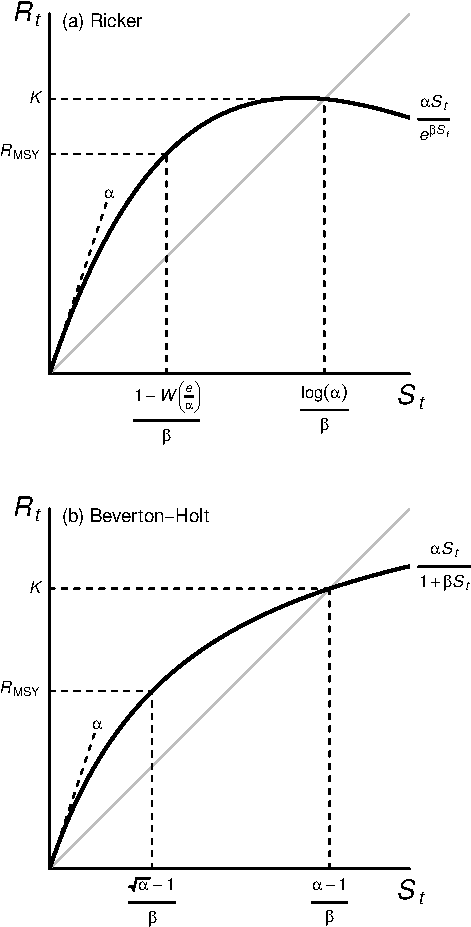
\includegraphics{App_3_Summarize_results_files/figure-latex/fig_1_model_forms-1} \end{center}

Figure 1. Deterministic forms of the (a) Ricker and (b) Beverton-Holt
models used in the analyses (thick lines), including equations for
carrying capacity (\(K\)) and the number of recruits corresponding to
the maximum sustained yield (RMSY). The parameter \(\alpha\) defines the
slope at the origin, the constant \(e\) is Euler's number, and \(W\) is
the Lambert function (see Scheuerell 2016 for details). The gray line is
where \(R_t = S_t\).

\hypertarget{main-results}{%
\section{Main results}\label{main-results}}

We need to convert the \texttt{mcmc.list} output into a more
user-friendly form for plotting, etc.

\begin{Shaded}
\begin{Highlighting}[]
\CommentTok{## results}
\NormalTok{mod_res <-}\StringTok{ }\KeywordTok{do.call}\NormalTok{(}\StringTok{"rbind"}\NormalTok{, best_fit)}
\end{Highlighting}
\end{Shaded}

\hypertarget{total-population-size}{%
\subsection{Total population size}\label{total-population-size}}

Here is our estimate of the total run size (i.e., catch + escapement)
over time, which includes a forecast for 2018. The black points are the
data, the blue line is the median posterior estimate, and the shaded
region is the 95\% credible interval. Note that the y-axis is on a log
scale.

\begin{Shaded}
\begin{Highlighting}[]
\NormalTok{clr <-}\StringTok{ }\KeywordTok{rgb}\NormalTok{(}\DecValTok{0}\NormalTok{, }\DecValTok{0}\NormalTok{, }\DecValTok{255}\NormalTok{, }\DataTypeTok{alpha =} \DecValTok{50}\NormalTok{, }\DataTypeTok{maxColorValue =} \DecValTok{255}\NormalTok{)}
\CommentTok{## estimated spawner data for plotting}
\NormalTok{p_dat <-}\StringTok{ }\NormalTok{mod_res[,}\KeywordTok{grep}\NormalTok{(}\StringTok{"Sp"}\NormalTok{, }\KeywordTok{colnames}\NormalTok{(mod_res))]}
\NormalTok{p_dat <-}\StringTok{ }\KeywordTok{apply}\NormalTok{(p_dat, }\DecValTok{2}\NormalTok{, quantile, CI_vec)}
\NormalTok{p_dat <-}\StringTok{ }\NormalTok{p_dat }\OperatorTok{+}\StringTok{ }\KeywordTok{matrix}\NormalTok{(dat_harv, }\KeywordTok{length}\NormalTok{(CI_vec), n_yrs}\OperatorTok{+}\NormalTok{n_fore, }\DataTypeTok{byrow =} \OtherTok{TRUE}\NormalTok{)}
\CommentTok{## time seq}
\NormalTok{t_idx_f <-}\StringTok{ }\KeywordTok{seq}\NormalTok{(yr_frst, }\DataTypeTok{length.out =}\NormalTok{ n_yrs}\OperatorTok{+}\NormalTok{n_fore)}
\CommentTok{## plot}
\NormalTok{yp_min <-}\StringTok{ }\KeywordTok{min}\NormalTok{(p_dat)}
\NormalTok{yp_max <-}\StringTok{ }\KeywordTok{max}\NormalTok{(p_dat)}
\KeywordTok{par}\NormalTok{(}\DataTypeTok{mai =} \KeywordTok{c}\NormalTok{(}\FloatTok{0.8}\NormalTok{,}\FloatTok{0.8}\NormalTok{,}\FloatTok{0.1}\NormalTok{,}\FloatTok{0.1}\NormalTok{), }\DataTypeTok{omi =} \KeywordTok{c}\NormalTok{(}\FloatTok{0.5}\NormalTok{,}\FloatTok{0.2}\NormalTok{,}\FloatTok{0.1}\NormalTok{,}\FloatTok{0.2}\NormalTok{))}
\KeywordTok{plot}\NormalTok{(t_idx_f, p_dat[}\DecValTok{3}\NormalTok{,], }\DataTypeTok{ylim =} \KeywordTok{c}\NormalTok{(yp_min,yp_max), }\DataTypeTok{type =} \StringTok{"n"}\NormalTok{,}
     \DataTypeTok{log =} \StringTok{"y"}\NormalTok{, }\DataTypeTok{xaxt =} \StringTok{"n"}\NormalTok{, }\DataTypeTok{yaxt =} \StringTok{"n"}\NormalTok{, }\DataTypeTok{bty =} \StringTok{"L"}\NormalTok{,}
     \DataTypeTok{xlab =} \StringTok{"Year"}\NormalTok{, }\DataTypeTok{ylab =} \StringTok{"Catch + escapement"}\NormalTok{, }\DataTypeTok{main =} \StringTok{""}\NormalTok{, }\DataTypeTok{cex.lab =} \FloatTok{1.2}\NormalTok{)}
\KeywordTok{polygon}\NormalTok{(}\KeywordTok{c}\NormalTok{(t_idx_f, }\KeywordTok{rev}\NormalTok{(t_idx_f)), }\KeywordTok{c}\NormalTok{(p_dat[}\DecValTok{3}\NormalTok{,], }\KeywordTok{rev}\NormalTok{(p_dat[}\DecValTok{1}\NormalTok{,])),}
        \DataTypeTok{col =}\NormalTok{ clr, }\DataTypeTok{border =} \OtherTok{NA}\NormalTok{)}
\KeywordTok{lines}\NormalTok{(t_idx_f, p_dat[}\DecValTok{2}\NormalTok{,], }\DataTypeTok{col =} \StringTok{"blue3"}\NormalTok{, }\DataTypeTok{lwd =} \DecValTok{2}\NormalTok{)}
\KeywordTok{points}\NormalTok{(t_idx_f, }\KeywordTok{exp}\NormalTok{(ln_dat_esc) }\OperatorTok{+}\StringTok{ }\NormalTok{dat_harv, }\DataTypeTok{pch =} \DecValTok{16}\NormalTok{, }\DataTypeTok{cex =} \DecValTok{1}\NormalTok{)}
\KeywordTok{axis}\NormalTok{(}\DecValTok{1}\NormalTok{, }\DataTypeTok{at =} \KeywordTok{seq}\NormalTok{(}\DecValTok{1980}\NormalTok{, }\DecValTok{2015}\NormalTok{, }\DecValTok{5}\NormalTok{))}
\KeywordTok{axis}\NormalTok{(}\DecValTok{2}\NormalTok{, }\DataTypeTok{at =} \KeywordTok{c}\NormalTok{(}\DecValTok{4000}\NormalTok{, }\DecValTok{8000}\NormalTok{, }\DecValTok{16000}\NormalTok{))}
\end{Highlighting}
\end{Shaded}

\begin{center}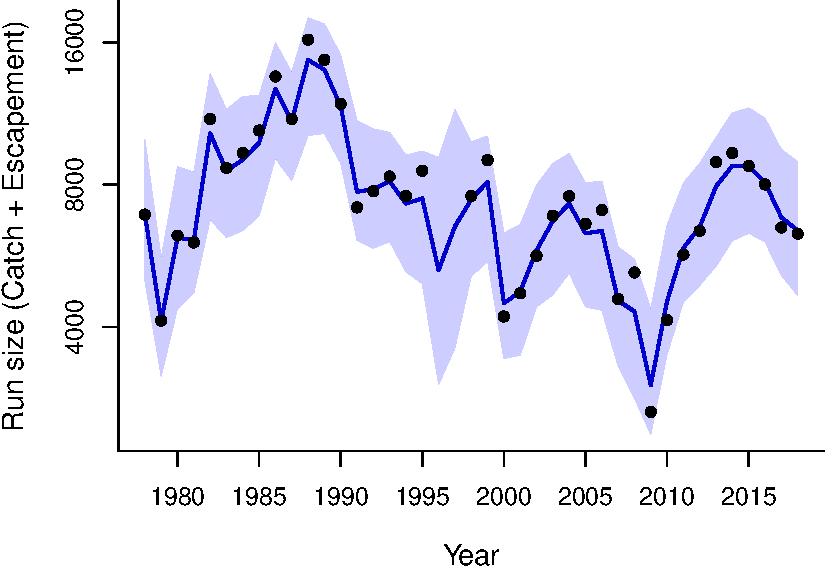
\includegraphics{App_3_Summarize_results_files/figure-latex/fig_2_run_size-1} \end{center}

Figure 2. Time series of the estimated total population size (catch plus
the adults that escaped to spawn). The observed data are the points; the
solid line is the median estimate and the shaded region indicates the
95\% credible interval.

\hypertarget{spawner-recruit-relationship}{%
\subsection{Spawner-recruit
relationship}\label{spawner-recruit-relationship}}

Here is the relationship between spawner and subsequent recruits (a),
assuming mean values for all covariates. Gray lines show the median
relationship for each of the 41 years based on \(a_t\). Note that for
plotting purposes only in (b) and (c), the density in the largest bin
for each parameter contains counts for all values greater or equal to
that. Vertical arrows under the x-axes in (b) and (c) indicate the
2.5\textsuperscript{th}, 50\textsuperscript{th}, and
97.5\textsuperscript{th} percentiles.

\begin{Shaded}
\begin{Highlighting}[]
\KeywordTok{layout}\NormalTok{(}\KeywordTok{matrix}\NormalTok{(}\KeywordTok{c}\NormalTok{(}\DecValTok{1}\NormalTok{,}\DecValTok{1}\NormalTok{,}\DecValTok{2}\NormalTok{,}\DecValTok{3}\NormalTok{),}\DecValTok{2}\NormalTok{,}\DecValTok{2}\NormalTok{),}\KeywordTok{c}\NormalTok{(}\DecValTok{3}\NormalTok{,}\DecValTok{2}\NormalTok{),}\KeywordTok{c}\NormalTok{(}\DecValTok{1}\NormalTok{,}\DecValTok{1}\NormalTok{))}
\NormalTok{xoffSet <-}\StringTok{ }\FloatTok{0.05}
\NormalTok{yoffSet <-}\StringTok{ }\FloatTok{0.03}

\CommentTok{## colors for plotting}
\NormalTok{clr <-}\StringTok{ }\KeywordTok{rgb}\NormalTok{(}\DecValTok{100}\NormalTok{, }\DecValTok{0}\NormalTok{, }\DecValTok{200}\NormalTok{,}
           \DataTypeTok{alpha =} \KeywordTok{seq}\NormalTok{(}\DecValTok{200}\NormalTok{, }\DecValTok{100}\NormalTok{,}
                       \DataTypeTok{length.out =}\NormalTok{ age_max}\OperatorTok{-}\NormalTok{age_min}\OperatorTok{+}\NormalTok{n_fore),}
           \DataTypeTok{maxColorValue =} \DecValTok{255}\NormalTok{)}

\CommentTok{## posterior of spawners}
\NormalTok{s_dat <-}\StringTok{ }\NormalTok{mod_res[,}\KeywordTok{grep}\NormalTok{(}\StringTok{"Sp"}\NormalTok{, }\KeywordTok{colnames}\NormalTok{(mod_res))]}
\NormalTok{s_dat <-}\StringTok{ }\KeywordTok{apply}\NormalTok{(s_dat, }\DecValTok{2}\NormalTok{, quantile, CI_vec)}
\NormalTok{s_dat <-}\StringTok{ }\NormalTok{s_dat[, }\DecValTok{1}\OperatorTok{:}\NormalTok{(n_yrs}\OperatorTok{-}\NormalTok{age_min}\OperatorTok{+}\NormalTok{n_fore)]}

\CommentTok{## posterior of recruits}
\NormalTok{r_dat <-}\StringTok{ }\NormalTok{mod_res[, }\KeywordTok{grep}\NormalTok{(}\StringTok{"tot_ln_Rec"}\NormalTok{, }\KeywordTok{colnames}\NormalTok{(mod_res))]}
\NormalTok{r_dat <-}\StringTok{ }\KeywordTok{exp}\NormalTok{(}\KeywordTok{apply}\NormalTok{(r_dat, }\DecValTok{2}\NormalTok{, quantile, CI_vec))}

\CommentTok{## median values for a & b}
\NormalTok{aa <-}\StringTok{ }\KeywordTok{apply}\NormalTok{(mod_res[, }\KeywordTok{grep}\NormalTok{(}\StringTok{"ln_BH_a"}\NormalTok{, }\KeywordTok{colnames}\NormalTok{(mod_res))], }\DecValTok{2}\NormalTok{, median)}
\NormalTok{bb <-}\StringTok{ }\KeywordTok{median}\NormalTok{(mod_res[, }\StringTok{"beta"}\NormalTok{])}

\CommentTok{## empty plot space for spawner-recruit relationships}
\NormalTok{dd <-}\StringTok{ }\DecValTok{3000}
\NormalTok{yM <-}\StringTok{ }\KeywordTok{Re2prec}\NormalTok{(}\KeywordTok{max}\NormalTok{(r_dat), }\StringTok{"ceiling"}\NormalTok{, dd)}
\NormalTok{xM <-}\StringTok{ }\KeywordTok{Re2prec}\NormalTok{(}\KeywordTok{max}\NormalTok{(s_dat), }\StringTok{"ceiling"}\NormalTok{, dd)}
\KeywordTok{par}\NormalTok{(}\DataTypeTok{mai =} \KeywordTok{c}\NormalTok{(}\FloatTok{0.8}\NormalTok{,}\FloatTok{0.8}\NormalTok{,}\FloatTok{0.1}\NormalTok{,}\FloatTok{0.1}\NormalTok{), }\DataTypeTok{omi =} \KeywordTok{c}\NormalTok{(}\DecValTok{0}\NormalTok{,}\DecValTok{0}\NormalTok{,}\DecValTok{0}\NormalTok{,}\DecValTok{0}\NormalTok{))}
\KeywordTok{plot}\NormalTok{(s_dat[}\DecValTok{2}\NormalTok{,], r_dat[}\DecValTok{2}\NormalTok{,], }\DataTypeTok{xlim =} \KeywordTok{c}\NormalTok{(}\DecValTok{0}\NormalTok{,xM), }\DataTypeTok{ylim =} \KeywordTok{c}\NormalTok{(}\DecValTok{0}\NormalTok{,yM), }\DataTypeTok{type =} \StringTok{"n"}\NormalTok{,}
     \DataTypeTok{xaxs =} \StringTok{"i"}\NormalTok{, }\DataTypeTok{yaxs =} \StringTok{"i"}\NormalTok{, }\DataTypeTok{cex.lab =} \FloatTok{1.2}\NormalTok{,}
     \DataTypeTok{xlab =} \KeywordTok{expression}\NormalTok{(Spawners}\OperatorTok{~}\NormalTok{(}\DecValTok{10}\OperatorTok{^}\DecValTok{3}\NormalTok{)),}
     \DataTypeTok{ylab =} \KeywordTok{expression}\NormalTok{(Recruits}\OperatorTok{~}\NormalTok{(}\DecValTok{10}\OperatorTok{^}\DecValTok{3}\NormalTok{)),}
     \DataTypeTok{xaxt =} \StringTok{"n"}\NormalTok{, }\DataTypeTok{yaxt =} \StringTok{"n"}\NormalTok{, }\DataTypeTok{bty=}\StringTok{"L"}\NormalTok{)}
\KeywordTok{axis}\NormalTok{(}\DecValTok{1}\NormalTok{, }\DataTypeTok{at =} \KeywordTok{seq}\NormalTok{(}\DecValTok{0}\NormalTok{,xM,dd}\OperatorTok{*}\DecValTok{2}\NormalTok{), }\DataTypeTok{labels =} \KeywordTok{seq}\NormalTok{(}\DecValTok{0}\NormalTok{,xM,dd}\OperatorTok{*}\DecValTok{2}\NormalTok{)}\OperatorTok{/}\DecValTok{1000}\NormalTok{)}
\KeywordTok{axis}\NormalTok{(}\DecValTok{2}\NormalTok{, }\DataTypeTok{at =} \KeywordTok{seq}\NormalTok{(}\DecValTok{0}\NormalTok{,yM,dd}\OperatorTok{*}\DecValTok{2}\NormalTok{), }\DataTypeTok{labels =} \KeywordTok{seq}\NormalTok{(}\DecValTok{0}\NormalTok{,yM,dd}\OperatorTok{*}\DecValTok{2}\NormalTok{)}\OperatorTok{/}\DecValTok{1000}\NormalTok{, }\DataTypeTok{las=}\DecValTok{1}\NormalTok{)}
\ControlFlowTok{for}\NormalTok{(i }\ControlFlowTok{in} \DecValTok{1}\OperatorTok{:}\KeywordTok{length}\NormalTok{(aa)) \{}
  \KeywordTok{lines}\NormalTok{(}\KeywordTok{exp}\NormalTok{(aa[i]) }\OperatorTok{*}\StringTok{ }\KeywordTok{seq}\NormalTok{(}\DecValTok{0}\NormalTok{,xM) }\OperatorTok{/}\StringTok{ }\NormalTok{(}\DecValTok{1} \OperatorTok{+}\StringTok{ }\NormalTok{bb }\OperatorTok{*}\StringTok{ }\KeywordTok{seq}\NormalTok{(}\DecValTok{0}\NormalTok{,xM)),}
        \DataTypeTok{col =} \StringTok{"darkgray"}\NormalTok{)}
\NormalTok{\}}
\KeywordTok{abline}\NormalTok{(}\DataTypeTok{a =} \DecValTok{0}\NormalTok{,}\DataTypeTok{b =} \DecValTok{1}\NormalTok{,}\DataTypeTok{lty =} \StringTok{"dashed"}\NormalTok{)}

\CommentTok{## add S-R estimates and medians}
\NormalTok{nCB <-}\StringTok{ }\NormalTok{n_yrs}\OperatorTok{-}\NormalTok{age_max}
\CommentTok{## years with complete returns}
\KeywordTok{points}\NormalTok{(s_dat[}\DecValTok{2}\NormalTok{, }\DecValTok{1}\OperatorTok{:}\NormalTok{nCB], r_dat[}\DecValTok{2}\NormalTok{, }\DecValTok{1}\OperatorTok{:}\NormalTok{nCB],}
       \DataTypeTok{xlim =} \KeywordTok{c}\NormalTok{(}\DecValTok{0}\NormalTok{,xM), }\DataTypeTok{ylim =} \KeywordTok{c}\NormalTok{(}\DecValTok{0}\NormalTok{,yM),}
       \DataTypeTok{pch =} \DecValTok{16}\NormalTok{, }\DataTypeTok{col =} \StringTok{"blue3"}\NormalTok{)}
\KeywordTok{segments}\NormalTok{(s_dat[}\DecValTok{2}\NormalTok{, }\DecValTok{1}\OperatorTok{:}\NormalTok{nCB], r_dat[}\DecValTok{1}\NormalTok{, }\DecValTok{1}\OperatorTok{:}\NormalTok{nCB],}
\NormalTok{         s_dat[}\DecValTok{2}\NormalTok{, }\DecValTok{1}\OperatorTok{:}\NormalTok{nCB], r_dat[}\DecValTok{3}\NormalTok{, }\DecValTok{1}\OperatorTok{:}\NormalTok{nCB],}
         \DataTypeTok{col =} \StringTok{"blue3"}\NormalTok{)}
\KeywordTok{segments}\NormalTok{(s_dat[}\DecValTok{1}\NormalTok{, }\DecValTok{1}\OperatorTok{:}\NormalTok{nCB], r_dat[}\DecValTok{2}\NormalTok{, }\DecValTok{1}\OperatorTok{:}\NormalTok{nCB],}
\NormalTok{         s_dat[}\DecValTok{3}\NormalTok{, }\DecValTok{1}\OperatorTok{:}\NormalTok{nCB], r_dat[}\DecValTok{2}\NormalTok{, }\DecValTok{1}\OperatorTok{:}\NormalTok{nCB],}
         \DataTypeTok{col =} \StringTok{"blue3"}\NormalTok{)}
\NormalTok{nTB <-}\StringTok{ }\KeywordTok{dim}\NormalTok{(s_dat)[}\DecValTok{2}\NormalTok{]}
\CommentTok{## years with incomplete returns}
\KeywordTok{segments}\NormalTok{(s_dat[}\DecValTok{2}\NormalTok{, (nCB}\OperatorTok{+}\DecValTok{1}\NormalTok{)}\OperatorTok{:}\NormalTok{nTB], r_dat[}\DecValTok{1}\NormalTok{, (nCB}\OperatorTok{+}\DecValTok{1}\NormalTok{)}\OperatorTok{:}\NormalTok{nTB],}
\NormalTok{         s_dat[}\DecValTok{2}\NormalTok{, (nCB}\OperatorTok{+}\DecValTok{1}\NormalTok{)}\OperatorTok{:}\NormalTok{nTB], r_dat[}\DecValTok{3}\NormalTok{, (nCB}\OperatorTok{+}\DecValTok{1}\NormalTok{)}\OperatorTok{:}\NormalTok{nTB],}
         \DataTypeTok{col =}\NormalTok{ clr)}
\KeywordTok{segments}\NormalTok{(s_dat[}\DecValTok{1}\NormalTok{, (nCB}\OperatorTok{+}\DecValTok{1}\NormalTok{)}\OperatorTok{:}\NormalTok{nTB], r_dat[}\DecValTok{2}\NormalTok{, (nCB}\OperatorTok{+}\DecValTok{1}\NormalTok{)}\OperatorTok{:}\NormalTok{nTB],}
\NormalTok{         s_dat[}\DecValTok{3}\NormalTok{, (nCB}\OperatorTok{+}\DecValTok{1}\NormalTok{)}\OperatorTok{:}\NormalTok{nTB], r_dat[}\DecValTok{2}\NormalTok{, (nCB}\OperatorTok{+}\DecValTok{1}\NormalTok{)}\OperatorTok{:}\NormalTok{nTB],}
         \DataTypeTok{col =}\NormalTok{ clr)}
\KeywordTok{points}\NormalTok{(s_dat[}\DecValTok{2}\NormalTok{, (nCB}\OperatorTok{+}\DecValTok{1}\NormalTok{)}\OperatorTok{:}\NormalTok{nTB],r_dat[}\DecValTok{2}\NormalTok{, (nCB}\OperatorTok{+}\DecValTok{1}\NormalTok{)}\OperatorTok{:}\NormalTok{nTB],}
       \DataTypeTok{xlim =} \KeywordTok{c}\NormalTok{(}\DecValTok{0}\NormalTok{,xM), }\DataTypeTok{ylim =} \KeywordTok{c}\NormalTok{(}\DecValTok{0}\NormalTok{,yM),}
       \DataTypeTok{pch =} \DecValTok{16}\NormalTok{, }\DataTypeTok{col =}\NormalTok{ clr)}
\KeywordTok{text}\NormalTok{(}\DataTypeTok{x =} \KeywordTok{par}\NormalTok{()}\OperatorTok{$}\NormalTok{usr[}\DecValTok{1}\NormalTok{] }\OperatorTok{+}\StringTok{ }\KeywordTok{diff}\NormalTok{(}\KeywordTok{par}\NormalTok{()}\OperatorTok{$}\NormalTok{usr[}\DecValTok{1}\OperatorTok{:}\DecValTok{2}\NormalTok{]) }\OperatorTok{*}\StringTok{ }\NormalTok{xoffSet,}
     \DataTypeTok{y =} \KeywordTok{par}\NormalTok{()}\OperatorTok{$}\NormalTok{usr[}\DecValTok{4}\NormalTok{] }\OperatorTok{-}\StringTok{ }\KeywordTok{diff}\NormalTok{(}\KeywordTok{par}\NormalTok{()}\OperatorTok{$}\NormalTok{usr[}\DecValTok{3}\OperatorTok{:}\DecValTok{4}\NormalTok{]) }\OperatorTok{*}\StringTok{ }\NormalTok{yoffSet,}
     \StringTok{"(a)"}\NormalTok{)}

\CommentTok{## posterior for alpha}
\NormalTok{clr <-}\StringTok{ }\KeywordTok{rgb}\NormalTok{(}\DecValTok{0}\NormalTok{, }\DecValTok{0}\NormalTok{, }\DecValTok{255}\NormalTok{, }\DataTypeTok{alpha =} \DecValTok{50}\NormalTok{, }\DataTypeTok{maxColorValue =} \DecValTok{255}\NormalTok{)}
\NormalTok{a_thresh <-}\StringTok{ }\DecValTok{59}
\KeywordTok{par}\NormalTok{(}\DataTypeTok{mai =} \KeywordTok{c}\NormalTok{(}\FloatTok{0.8}\NormalTok{,}\FloatTok{0.4}\NormalTok{,}\FloatTok{0.3}\NormalTok{,}\FloatTok{0.1}\NormalTok{))}
\CommentTok{## B-H alpha}
\NormalTok{R_alpha_est <-}\StringTok{ }\NormalTok{mod_res[, }\StringTok{"alpha"}\NormalTok{]}
\NormalTok{alphaCI <-}\StringTok{ }\KeywordTok{quantile}\NormalTok{(R_alpha_est, CI_vec)}
\NormalTok{R_alpha_est[R_alpha_est }\OperatorTok{>}\StringTok{ }\NormalTok{a_thresh] <-}\StringTok{ }\NormalTok{a_thresh}
\KeywordTok{hist}\NormalTok{(R_alpha_est, }\DataTypeTok{freq =} \OtherTok{FALSE}\NormalTok{, }\DataTypeTok{breaks =} \KeywordTok{seq}\NormalTok{(}\DecValTok{0}\NormalTok{, a_thresh}\OperatorTok{+}\DecValTok{1}\NormalTok{, }\DecValTok{2}\NormalTok{),}
     \DataTypeTok{col =}\NormalTok{ clr, }\DataTypeTok{border =} \StringTok{"blue3"}\NormalTok{,}
     \DataTypeTok{xlab =} \StringTok{""}\NormalTok{, }\DataTypeTok{ylab =} \StringTok{""}\NormalTok{, }\DataTypeTok{main =} \StringTok{""}\NormalTok{, }\DataTypeTok{cex.lab =} \FloatTok{1.2}\NormalTok{, }\DataTypeTok{yaxt =} \StringTok{"n"}\NormalTok{)}
\NormalTok{aHt <-}\StringTok{ }\NormalTok{(}\KeywordTok{par}\NormalTok{()}\OperatorTok{$}\NormalTok{usr[}\DecValTok{4}\NormalTok{]}\OperatorTok{-}\KeywordTok{par}\NormalTok{()}\OperatorTok{$}\NormalTok{usr[}\DecValTok{3}\NormalTok{])}\OperatorTok{/}\DecValTok{12}
\KeywordTok{arrows}\NormalTok{(alphaCI, }\KeywordTok{par}\NormalTok{()}\OperatorTok{$}\NormalTok{usr[}\DecValTok{3}\NormalTok{], alphaCI,}\KeywordTok{par}\NormalTok{()}\OperatorTok{$}\NormalTok{usr[}\DecValTok{3}\NormalTok{]}\OperatorTok{-}\NormalTok{aHt,}
       \DataTypeTok{code =} \DecValTok{1}\NormalTok{, }\DataTypeTok{length =} \FloatTok{0.05}\NormalTok{, }\DataTypeTok{xpd =} \OtherTok{NA}\NormalTok{, }\DataTypeTok{col =} \StringTok{"blue3"}\NormalTok{, }\DataTypeTok{lwd =} \FloatTok{1.5}\NormalTok{)}
\KeywordTok{mtext}\NormalTok{(}\KeywordTok{expression}\NormalTok{(Instrinsic}\OperatorTok{~}\NormalTok{productivity}\OperatorTok{~}\NormalTok{(alpha)), }\DecValTok{1}\NormalTok{, }\DataTypeTok{line =} \DecValTok{3}\NormalTok{, }\DataTypeTok{cex =} \DecValTok{1}\NormalTok{)}
\KeywordTok{text}\NormalTok{(}\DataTypeTok{x =} \KeywordTok{par}\NormalTok{()}\OperatorTok{$}\NormalTok{usr[}\DecValTok{1}\NormalTok{],}
     \DataTypeTok{y =} \KeywordTok{par}\NormalTok{()}\OperatorTok{$}\NormalTok{usr[}\DecValTok{4}\NormalTok{] }\OperatorTok{*}\StringTok{ }\FloatTok{1.05}\NormalTok{,}
     \StringTok{"(b)"}\NormalTok{, }\DataTypeTok{xpd=}\OtherTok{NA}\NormalTok{)}

\CommentTok{## posterior for K}
\KeywordTok{par}\NormalTok{(}\DataTypeTok{mai =} \KeywordTok{c}\NormalTok{(}\FloatTok{0.8}\NormalTok{,}\FloatTok{0.4}\NormalTok{,}\FloatTok{0.3}\NormalTok{,}\FloatTok{0.1}\NormalTok{))}
\NormalTok{aa <-}\StringTok{ }\NormalTok{mod_res[, }\StringTok{"alpha"}\NormalTok{]}
\NormalTok{bb <-}\StringTok{ }\NormalTok{mod_res[, }\StringTok{"beta"}\NormalTok{]}
\CommentTok{## K in 1000s}
\NormalTok{R_b_est <-}\StringTok{ }\NormalTok{(aa}\DecValTok{-1}\NormalTok{) }\OperatorTok{/}\StringTok{ }\NormalTok{bb }\OperatorTok{/}\StringTok{ }\DecValTok{1000}
\NormalTok{R_b_est <-}\StringTok{ }\NormalTok{R_b_est[R_b_est }\OperatorTok{>}\StringTok{ }\DecValTok{0}\NormalTok{]}
\NormalTok{R_b_CI <-}\StringTok{ }\KeywordTok{quantile}\NormalTok{(R_b_est, CI_vec)}
\CommentTok{## pile into last ban for plotting}
\NormalTok{R_b_est[R_b_est }\OperatorTok{>}\StringTok{ }\DecValTok{13}\NormalTok{] <-}\StringTok{ }\DecValTok{13}
\NormalTok{brks <-}\StringTok{ }\KeywordTok{seq}\NormalTok{(}\KeywordTok{Re2prec}\NormalTok{(}\KeywordTok{min}\NormalTok{(R_b_est), }\StringTok{"floor"}\NormalTok{),}
            \KeywordTok{Re2prec}\NormalTok{(}\KeywordTok{max}\NormalTok{(R_b_est), }\StringTok{"ceiling"}\NormalTok{),}
            \DataTypeTok{length.out =} \KeywordTok{length}\NormalTok{(}\KeywordTok{seq}\NormalTok{(}\DecValTok{0}\NormalTok{, a_thresh, }\DecValTok{2}\NormalTok{)))}
\KeywordTok{hist}\NormalTok{(R_b_est, }\DataTypeTok{freq =} \OtherTok{FALSE}\NormalTok{, }\DataTypeTok{breaks =}\NormalTok{ brks, }\DataTypeTok{col =}\NormalTok{ clr, }\DataTypeTok{border =} \StringTok{"blue3"}\NormalTok{,}
     \DataTypeTok{xlab =} \StringTok{""}\NormalTok{, }\DataTypeTok{xaxt =} \StringTok{"n"}\NormalTok{, }\DataTypeTok{yaxt =} \StringTok{"n"}\NormalTok{,}
     \DataTypeTok{main =} \StringTok{""}\NormalTok{, }\DataTypeTok{ylab =} \StringTok{""}\NormalTok{, }\DataTypeTok{cex.lab =} \FloatTok{1.2}\NormalTok{)}
\KeywordTok{axis}\NormalTok{(}\DecValTok{1}\NormalTok{, }\DataTypeTok{at =} \KeywordTok{seq}\NormalTok{(}\KeywordTok{Re2prec}\NormalTok{(}\KeywordTok{min}\NormalTok{(R_b_est), }\StringTok{"floor"}\NormalTok{),}
                 \KeywordTok{Re2prec}\NormalTok{(}\KeywordTok{max}\NormalTok{(R_b_est), }\StringTok{"ceiling"}\NormalTok{),}
                 \DecValTok{2}\NormalTok{))}
\NormalTok{aHt <-}\StringTok{ }\NormalTok{(}\KeywordTok{par}\NormalTok{()}\OperatorTok{$}\NormalTok{usr[}\DecValTok{4}\NormalTok{] }\OperatorTok{-}\StringTok{ }\KeywordTok{par}\NormalTok{()}\OperatorTok{$}\NormalTok{usr[}\DecValTok{3}\NormalTok{]) }\OperatorTok{/}\StringTok{ }\DecValTok{12}
\KeywordTok{arrows}\NormalTok{(R_b_CI, }\KeywordTok{par}\NormalTok{()}\OperatorTok{$}\NormalTok{usr[}\DecValTok{3}\NormalTok{], R_b_CI,}\KeywordTok{par}\NormalTok{()}\OperatorTok{$}\NormalTok{usr[}\DecValTok{3}\NormalTok{]}\OperatorTok{-}\NormalTok{aHt,}
       \DataTypeTok{code =} \DecValTok{1}\NormalTok{, }\DataTypeTok{length =} \FloatTok{0.05}\NormalTok{, }\DataTypeTok{xpd =} \OtherTok{NA}\NormalTok{, }\DataTypeTok{col =} \StringTok{"blue3"}\NormalTok{, }\DataTypeTok{lwd =} \FloatTok{1.5}\NormalTok{)}
\KeywordTok{mtext}\NormalTok{(}\KeywordTok{expression}\NormalTok{(}\KeywordTok{paste}\NormalTok{(}\StringTok{"Carrying capacity ("}\NormalTok{,}\KeywordTok{italic}\NormalTok{(K),}\StringTok{", "}\NormalTok{,}\DecValTok{10}\OperatorTok{^}\DecValTok{3}\NormalTok{,}\StringTok{")"}\NormalTok{)),}
      \DataTypeTok{side =} \DecValTok{1}\NormalTok{, }\DataTypeTok{line =} \DecValTok{3}\NormalTok{, }\DataTypeTok{cex =} \DecValTok{1}\NormalTok{)}
\KeywordTok{text}\NormalTok{(}\DataTypeTok{x =} \KeywordTok{par}\NormalTok{()}\OperatorTok{$}\NormalTok{usr[}\DecValTok{1}\NormalTok{], }
     \DataTypeTok{y =} \KeywordTok{par}\NormalTok{()}\OperatorTok{$}\NormalTok{usr[}\DecValTok{4}\NormalTok{] }\OperatorTok{*}\StringTok{ }\FloatTok{1.05}\NormalTok{,}
     \StringTok{"(c)"}\NormalTok{, }\DataTypeTok{xpd=}\OtherTok{NA}\NormalTok{)}
\end{Highlighting}
\end{Shaded}

\begin{center}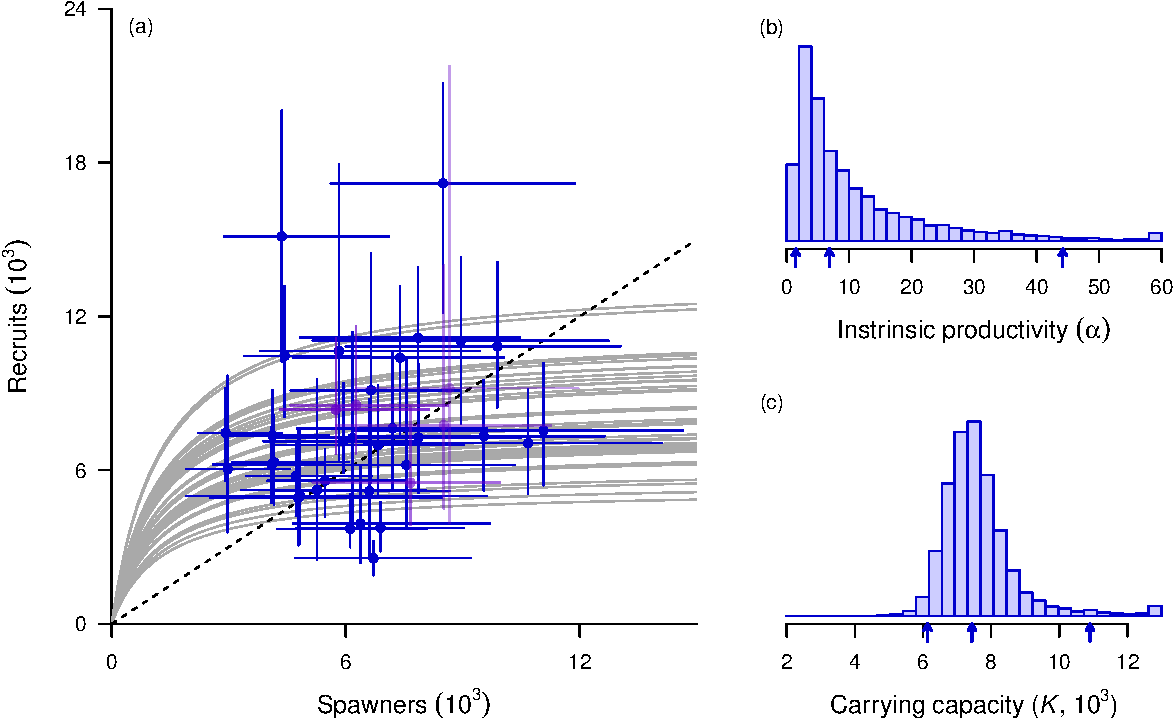
\includegraphics{App_3_Summarize_results_files/figure-latex/fig_3_S-R-1} \end{center}

Figure 3. Relationship between the number of spawning adults and their
subsequent surviving offspring (recruits), assuming mean values for all
covariates (a); and the estimated posterior distributions for the
intrinsic productivity (b) and carrying capacity (c). Points in (a) are
medians of the posterior estimates; error bars indicate the 95\%
credible intervals. Blue points are for estimates with complete broods;
purple points are for the most recent years with incomplete broods. Gray
lines show the median relationship for each of the 41 years in the time
series based on annual model estimates of productivity. Note that for
plotting purposes only in (b) and (c), the density in the largest bin
for each parameter contains counts for all values greater than or equal
to it. Vertical arrows under the x-axes in (b) and (c) indicate the
2.5\(^\text{th}\), 50\(^\text{th}\), and 97.5\(^\text{th}\) percentiles.

\hypertarget{covariate-effects}{%
\subsection{Covariate effects}\label{covariate-effects}}

Here are time series plots of the covariates (a-c) and histograms of
their effects on productivity (d-f).

\begin{Shaded}
\begin{Highlighting}[]
\NormalTok{clr <-}\StringTok{ }\KeywordTok{rgb}\NormalTok{(}\DecValTok{0}\NormalTok{, }\DecValTok{0}\NormalTok{, }\DecValTok{255}\NormalTok{, }\DataTypeTok{alpha =} \DecValTok{50}\NormalTok{, }\DataTypeTok{maxColorValue =} \DecValTok{255}\NormalTok{)}
\NormalTok{xoffSet <-}\StringTok{ }\FloatTok{0.04}
\NormalTok{yoffSet <-}\StringTok{ }\FloatTok{0.03}

\KeywordTok{par}\NormalTok{(}\DataTypeTok{mfrow=}\KeywordTok{c}\NormalTok{(n_cov,}\DecValTok{2}\NormalTok{), }\DataTypeTok{mai=}\KeywordTok{c}\NormalTok{(}\FloatTok{0.4}\NormalTok{,}\FloatTok{0.2}\NormalTok{,}\FloatTok{0.1}\NormalTok{,}\FloatTok{0.1}\NormalTok{), }\DataTypeTok{omi=}\KeywordTok{c}\NormalTok{(}\FloatTok{0.2}\NormalTok{,}\FloatTok{0.5}\NormalTok{,}\DecValTok{0}\NormalTok{,}\DecValTok{0}\NormalTok{))}

\NormalTok{c_est <-}\StringTok{ }\NormalTok{mod_res[,}\KeywordTok{grep}\NormalTok{(}\StringTok{"gamma"}\NormalTok{, }\KeywordTok{colnames}\NormalTok{(mod_res))]}
\NormalTok{ylN <-}\StringTok{ }\KeywordTok{floor}\NormalTok{(}\KeywordTok{min}\NormalTok{(c_est)}\OperatorTok{*}\DecValTok{10}\NormalTok{)}\OperatorTok{/}\DecValTok{10}
\NormalTok{ylM <-}\StringTok{ }\KeywordTok{ceiling}\NormalTok{(}\KeywordTok{max}\NormalTok{(c_est)}\OperatorTok{*}\DecValTok{10}\NormalTok{)}\OperatorTok{/}\DecValTok{10}
\NormalTok{brks <-}\StringTok{ }\KeywordTok{seq}\NormalTok{(ylN,ylM,}\DataTypeTok{length.out=}\KeywordTok{diff}\NormalTok{(}\KeywordTok{c}\NormalTok{(ylN,ylM))}\OperatorTok{*}\DecValTok{40}\OperatorTok{+}\DecValTok{1}\NormalTok{)}
\NormalTok{t_idx <-}\StringTok{ }\KeywordTok{seq}\NormalTok{(yr_frst,}\DataTypeTok{length.out=}\NormalTok{n_yrs}\OperatorTok{-}\NormalTok{age_min}\OperatorTok{+}\NormalTok{n_fore)}
\NormalTok{dat_cvrs <-}\StringTok{ }\KeywordTok{as.matrix}\NormalTok{(dat_cvrs[}\KeywordTok{seq}\NormalTok{(}\KeywordTok{length}\NormalTok{(t_idx)),])}

\ControlFlowTok{for}\NormalTok{(i }\ControlFlowTok{in} \DecValTok{1}\OperatorTok{:}\NormalTok{n_cov) \{}
  \ControlFlowTok{if}\NormalTok{(i}\OperatorTok{==}\DecValTok{4}\NormalTok{) \{}
\NormalTok{    dat_cvrs[,i}\OperatorTok{+}\DecValTok{1}\NormalTok{] <-}\StringTok{ }\NormalTok{dat_cvrs[,i}\OperatorTok{+}\DecValTok{1}\NormalTok{]}\OperatorTok{/}\DecValTok{1000}
\NormalTok{  \}}
  \CommentTok{## plot covar ts}
  \KeywordTok{plot}\NormalTok{(dat_cvrs[, }\StringTok{"year"}\NormalTok{], dat_cvrs[, i}\OperatorTok{+}\DecValTok{1}\NormalTok{],}
       \DataTypeTok{pch =} \DecValTok{16}\NormalTok{, }\DataTypeTok{col =} \StringTok{"blue3"}\NormalTok{, }\DataTypeTok{type =} \StringTok{"o"}\NormalTok{,}
       \DataTypeTok{xlab =} \StringTok{""}\NormalTok{, }\DataTypeTok{ylab =} \StringTok{""}\NormalTok{, }\DataTypeTok{main =} \StringTok{""}\NormalTok{, }\DataTypeTok{bty =} \StringTok{"L"}\NormalTok{,}
       \DataTypeTok{cex.axis =} \FloatTok{1.2}\NormalTok{)}
  \KeywordTok{text}\NormalTok{(}\DataTypeTok{x =} \KeywordTok{par}\NormalTok{()}\OperatorTok{$}\NormalTok{usr[}\DecValTok{1}\NormalTok{] }\OperatorTok{+}\StringTok{ }\KeywordTok{diff}\NormalTok{(}\KeywordTok{par}\NormalTok{()}\OperatorTok{$}\NormalTok{usr[}\DecValTok{1}\OperatorTok{:}\DecValTok{2}\NormalTok{]) }\OperatorTok{*}\StringTok{ }\NormalTok{xoffSet,}
       \DataTypeTok{y =} \KeywordTok{par}\NormalTok{()}\OperatorTok{$}\NormalTok{usr[}\DecValTok{4}\NormalTok{] }\OperatorTok{-}\StringTok{ }\KeywordTok{diff}\NormalTok{(}\KeywordTok{par}\NormalTok{()}\OperatorTok{$}\NormalTok{usr[}\DecValTok{3}\OperatorTok{:}\DecValTok{4}\NormalTok{]) }\OperatorTok{*}\StringTok{ }\NormalTok{yoffSet,}
       \KeywordTok{paste0}\NormalTok{(}\StringTok{"("}\NormalTok{,letters[i],}\StringTok{")"}\NormalTok{),}
       \DataTypeTok{cex =} \FloatTok{1.2}\NormalTok{)}
  \KeywordTok{mtext}\NormalTok{(}\DataTypeTok{side =} \DecValTok{2}\NormalTok{, cov_names[i], }\DataTypeTok{line =} \DecValTok{3}\NormalTok{, }\DataTypeTok{cex =} \FloatTok{1.2}\NormalTok{)}
  \ControlFlowTok{if}\NormalTok{(i }\OperatorTok{==}\StringTok{ }\NormalTok{n_cov) \{}
    \KeywordTok{mtext}\NormalTok{(}\DataTypeTok{side =} \DecValTok{1}\NormalTok{, }\StringTok{"Brood year"}\NormalTok{, }\DataTypeTok{line =} \DecValTok{3}\NormalTok{)}
\NormalTok{  \}}
  \CommentTok{## plot covar effect}
  \KeywordTok{hist}\NormalTok{(c_est[,i],}
       \DataTypeTok{freq =} \OtherTok{FALSE}\NormalTok{, }\DataTypeTok{breaks =}\NormalTok{ brks, }\DataTypeTok{col =}\NormalTok{ clr, }\DataTypeTok{border =}\StringTok{" blue3"}\NormalTok{,}
       \DataTypeTok{xlab =} \StringTok{""}\NormalTok{, }\DataTypeTok{yaxt =} \StringTok{"n"}\NormalTok{, }\DataTypeTok{main =} \StringTok{""}\NormalTok{, }\DataTypeTok{ylab =} \StringTok{""}\NormalTok{, }\DataTypeTok{cex.axis =} \FloatTok{1.2}\NormalTok{)}
\NormalTok{  c_CI <-}\StringTok{ }\KeywordTok{quantile}\NormalTok{(c_est[,i],CI_vec)}
\NormalTok{  aHt <-}\StringTok{ }\NormalTok{(}\KeywordTok{par}\NormalTok{()}\OperatorTok{$}\NormalTok{usr[}\DecValTok{4}\NormalTok{]}\OperatorTok{-}\KeywordTok{par}\NormalTok{()}\OperatorTok{$}\NormalTok{usr[}\DecValTok{3}\NormalTok{])}\OperatorTok{/}\DecValTok{20}
  \KeywordTok{arrows}\NormalTok{(c_CI, }\KeywordTok{par}\NormalTok{()}\OperatorTok{$}\NormalTok{usr[}\DecValTok{3}\NormalTok{]}\OperatorTok{-}\FloatTok{0.005}\NormalTok{, c_CI, }\KeywordTok{par}\NormalTok{()}\OperatorTok{$}\NormalTok{usr[}\DecValTok{3}\NormalTok{] }\OperatorTok{-}\StringTok{ }\NormalTok{aHt,}
         \DataTypeTok{code =} \DecValTok{1}\NormalTok{,}\DataTypeTok{length =} \FloatTok{0.05}\NormalTok{, }\DataTypeTok{xpd =} \OtherTok{NA}\NormalTok{, }\DataTypeTok{col =} \StringTok{"blue3"}\NormalTok{, }\DataTypeTok{lwd =} \FloatTok{1.5}\NormalTok{)}
  \KeywordTok{abline}\NormalTok{(}\DataTypeTok{v =} \DecValTok{0}\NormalTok{, }\DataTypeTok{lty =} \StringTok{"dashed"}\NormalTok{)}
  \KeywordTok{text}\NormalTok{(}\DataTypeTok{x =} \KeywordTok{par}\NormalTok{()}\OperatorTok{$}\NormalTok{usr[}\DecValTok{1}\NormalTok{] }\OperatorTok{+}\StringTok{ }\KeywordTok{diff}\NormalTok{(}\KeywordTok{par}\NormalTok{()}\OperatorTok{$}\NormalTok{usr[}\DecValTok{1}\OperatorTok{:}\DecValTok{2}\NormalTok{]) }\OperatorTok{*}\StringTok{ }\NormalTok{xoffSet,}
       \DataTypeTok{y =} \KeywordTok{par}\NormalTok{()}\OperatorTok{$}\NormalTok{usr[}\DecValTok{4}\NormalTok{] }\OperatorTok{-}\StringTok{ }\KeywordTok{diff}\NormalTok{(}\KeywordTok{par}\NormalTok{()}\OperatorTok{$}\NormalTok{usr[}\DecValTok{3}\OperatorTok{:}\DecValTok{4}\NormalTok{]) }\OperatorTok{*}\StringTok{ }\NormalTok{yoffSet,}
       \KeywordTok{paste0}\NormalTok{(}\StringTok{"("}\NormalTok{,letters[i}\OperatorTok{+}\NormalTok{n_cov],}\StringTok{")"}\NormalTok{),}
       \DataTypeTok{cex =} \FloatTok{1.2}\NormalTok{)}
  \ControlFlowTok{if}\NormalTok{(i }\OperatorTok{==}\StringTok{ }\NormalTok{n_cov) \{ }\KeywordTok{mtext}\NormalTok{(}\DataTypeTok{side =} \DecValTok{1}\NormalTok{,}\StringTok{"Effect size"}\NormalTok{, }\DataTypeTok{line =} \DecValTok{3}\NormalTok{) \}}
\NormalTok{\}}
\end{Highlighting}
\end{Shaded}

\begin{center}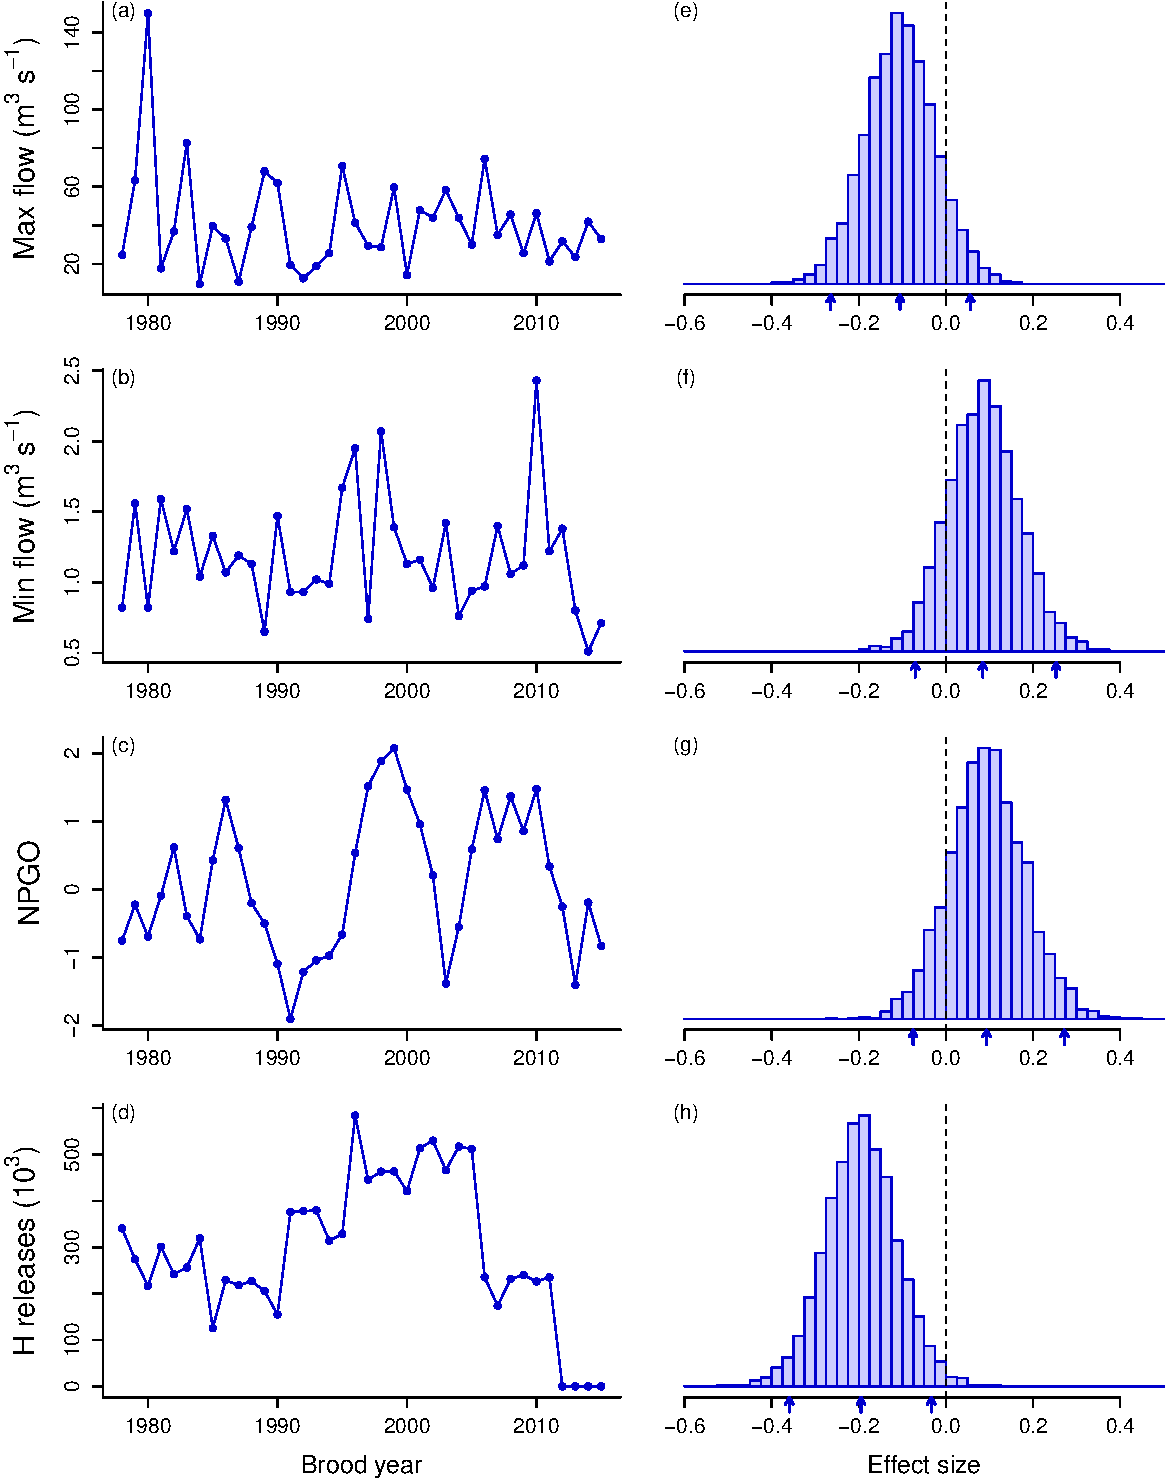
\includegraphics{App_3_Summarize_results_files/figure-latex/fig_4_cov_effects-1} \end{center}

Figure 4. Time series of the environmental covariates used in the model
(a-d), and their estimated effects on population productivity (e-g).
Small arrows under histograms denote 2.5\(^\text{th}\),
50\(^\text{th}\), and 97.5\(^\text{th}\) percentiles of the posterior
distribution.

\hypertarget{process-errors}{%
\subsection{Process errors}\label{process-errors}}

Here is the time series of the residuals from the process model. They
represent the population's productivity after accounting for the effects
of density dependence and environmental covariates.

\begin{Shaded}
\begin{Highlighting}[]
\CommentTok{## time sequence}
\NormalTok{t_idx_a <-}\StringTok{ }\KeywordTok{seq}\NormalTok{(yr_frst, }\DataTypeTok{length.out =}\NormalTok{ n_yrs}\OperatorTok{-}\NormalTok{age_min}\OperatorTok{+}\NormalTok{n_fore)}
\CommentTok{## plot data}
\NormalTok{p_dat <-}\StringTok{ }\NormalTok{mod_res[, }\KeywordTok{grep}\NormalTok{(}\StringTok{"res_ln_Rec"}\NormalTok{, }\KeywordTok{colnames}\NormalTok{(mod_res))]}
\NormalTok{p_dat <-}\StringTok{ }\KeywordTok{apply}\NormalTok{(p_dat, }\DecValTok{2}\NormalTok{, quantile, CI_vec)}
\NormalTok{yp_min <-}\StringTok{ }\KeywordTok{min}\NormalTok{(p_dat)}
\NormalTok{yp_max <-}\StringTok{ }\KeywordTok{max}\NormalTok{(p_dat)}
\CommentTok{## plot}
\KeywordTok{par}\NormalTok{(}\DataTypeTok{mai =} \KeywordTok{c}\NormalTok{(}\FloatTok{0.8}\NormalTok{,}\FloatTok{0.8}\NormalTok{,}\FloatTok{0.1}\NormalTok{,}\FloatTok{0.1}\NormalTok{), }\DataTypeTok{omi =} \KeywordTok{c}\NormalTok{(}\DecValTok{0}\NormalTok{,}\FloatTok{0.2}\NormalTok{,}\FloatTok{0.1}\NormalTok{,}\FloatTok{0.2}\NormalTok{))}
\KeywordTok{plot}\NormalTok{(t_idx_a, p_dat[}\DecValTok{3}\NormalTok{,],}
     \DataTypeTok{type =} \StringTok{"n"}\NormalTok{,  }\DataTypeTok{bty =} \StringTok{"L"}\NormalTok{,}
     \DataTypeTok{ylim =} \KeywordTok{c}\NormalTok{(yp_min,yp_max),}
     \DataTypeTok{xlab =} \StringTok{"Brood year"}\NormalTok{, }\DataTypeTok{ylab =} \StringTok{"Process error"}\NormalTok{, }\DataTypeTok{main =} \StringTok{""}\NormalTok{,}
     \DataTypeTok{cex.lab =} \FloatTok{1.2}\NormalTok{)}
\KeywordTok{abline}\NormalTok{(}\DataTypeTok{h =} \DecValTok{0}\NormalTok{, }\DataTypeTok{lty =} \StringTok{"dashed"}\NormalTok{)}
\KeywordTok{polygon}\NormalTok{(}\KeywordTok{c}\NormalTok{(t_idx_a, }\KeywordTok{rev}\NormalTok{(t_idx_a)), }\KeywordTok{c}\NormalTok{(p_dat[}\DecValTok{3}\NormalTok{,], }\KeywordTok{rev}\NormalTok{(p_dat[}\DecValTok{1}\NormalTok{,])),}
        \DataTypeTok{col =}\NormalTok{ clr, }\DataTypeTok{border =} \OtherTok{NA}\NormalTok{)}
\KeywordTok{lines}\NormalTok{(t_idx_a, p_dat[}\DecValTok{2}\NormalTok{,], }\DataTypeTok{col =} \StringTok{"blue3"}\NormalTok{, }\DataTypeTok{lwd =} \DecValTok{2}\NormalTok{)}
\end{Highlighting}
\end{Shaded}

\begin{center}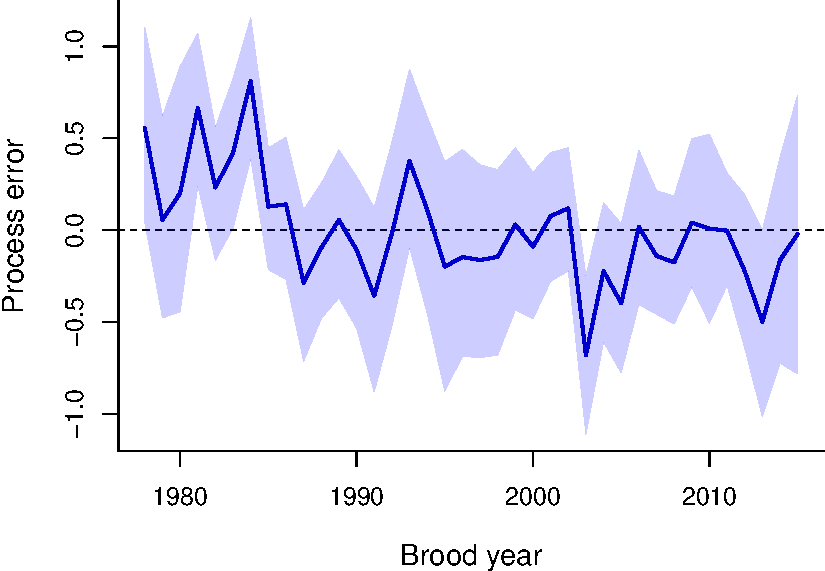
\includegraphics{App_3_Summarize_results_files/figure-latex/fig_5_proc_err-1} \end{center}

Figure 5. Time series of the estimated process errors, which represent
the population's productivity after accounting for the effects of
density dependence and environmental covariates. The solid line is the
median estimate and the shaded region indicates the 95\% credible
interval.

\hypertarget{management-reference-points}{%
\subsection{Management reference
points}\label{management-reference-points}}

Here are a number of management reference points.

\begin{Shaded}
\begin{Highlighting}[]
\CommentTok{## abbreviations for ref points}
\NormalTok{ref_names <-}\StringTok{ }\KeywordTok{c}\NormalTok{(}\StringTok{"MSY"}\NormalTok{, }\StringTok{"Smsy"}\NormalTok{, }\StringTok{"Umsy"}\NormalTok{, }\StringTok{"Umax"}\NormalTok{)}
\CommentTok{## proportions of MSY to consider}
\NormalTok{yld_prop <-}\StringTok{ }\KeywordTok{c}\NormalTok{(}\FloatTok{0.75}\NormalTok{, }\FloatTok{0.85}\NormalTok{, }\FloatTok{0.95}\NormalTok{)}
\CommentTok{## median values for a & b}
\NormalTok{aa <-}\StringTok{ }\NormalTok{mod_res[, }\KeywordTok{grep}\NormalTok{(}\StringTok{"E_BH_a"}\NormalTok{, }\KeywordTok{colnames}\NormalTok{(mod_res))]}
\NormalTok{alpha <-}\StringTok{ }\KeywordTok{exp}\NormalTok{(aa)}
\NormalTok{mcmc <-}\StringTok{ }\KeywordTok{length}\NormalTok{(aa)}
\NormalTok{beta <-}\StringTok{ }\NormalTok{mod_res[, }\KeywordTok{grep}\NormalTok{(}\StringTok{"beta"}\NormalTok{, }\KeywordTok{colnames}\NormalTok{(mod_res))]}

\CommentTok{## empty matrix for ref pts}
\NormalTok{ref_pts <-}\StringTok{ }\KeywordTok{matrix}\NormalTok{(}\OtherTok{NA}\NormalTok{, mcmc, }\KeywordTok{length}\NormalTok{(ref_names))}
\KeywordTok{colnames}\NormalTok{(ref_pts) <-}\StringTok{ }\NormalTok{ref_names}
\CommentTok{## spawner series for optimal yield profile}
\NormalTok{SS <-}\StringTok{ }\KeywordTok{seq}\NormalTok{(}\DecValTok{100}\NormalTok{, }\FloatTok{1e4}\NormalTok{, }\DecValTok{100}\NormalTok{)}
\CommentTok{## empty matrix for optimal yield profiles}
\NormalTok{OYP <-}\StringTok{ }\KeywordTok{matrix}\NormalTok{(}\DecValTok{0}\NormalTok{, }\KeywordTok{length}\NormalTok{(SS), }\KeywordTok{length}\NormalTok{(yld_prop))}
\ControlFlowTok{for}\NormalTok{(i }\ControlFlowTok{in} \DecValTok{1}\OperatorTok{:}\NormalTok{mcmc) \{}
    \CommentTok{## spawners at MSY}
\NormalTok{    ref_pts[i, }\StringTok{"Smsy"}\NormalTok{] <-}\StringTok{ }\NormalTok{(alpha[i] }\OperatorTok{/}\StringTok{ }\NormalTok{beta[i]) }\OperatorTok{*}\StringTok{ }\KeywordTok{sqrt}\NormalTok{(}\DecValTok{1} \OperatorTok{/}\StringTok{ }\NormalTok{alpha[i]) }\OperatorTok{-}\StringTok{ }\NormalTok{(}\DecValTok{1} \OperatorTok{/}\StringTok{ }\NormalTok{beta[i])}
    \CommentTok{## MSY}
\NormalTok{    ref_pts[i, }\StringTok{"MSY"}\NormalTok{] <-}\StringTok{ }\NormalTok{(ref_pts[i,}\StringTok{"Smsy"}\NormalTok{] }\OperatorTok{*}\StringTok{ }\NormalTok{alpha[i]) }\OperatorTok{/}
\StringTok{                            }\NormalTok{(}\DecValTok{1} \OperatorTok{+}\StringTok{ }\NormalTok{beta[i] }\OperatorTok{*}\StringTok{ }\NormalTok{ref_pts[i, }\StringTok{"Smsy"}\NormalTok{]) }\OperatorTok{-}\StringTok{ }\NormalTok{ref_pts[i, }\StringTok{"Smsy"}\NormalTok{]}
    \CommentTok{## harvest rate at MSY}
\NormalTok{    ref_pts[i, }\StringTok{"Umsy"}\NormalTok{] <-}\StringTok{ }\DecValTok{1} \OperatorTok{-}\StringTok{ }\KeywordTok{sqrt}\NormalTok{(}\DecValTok{1} \OperatorTok{/}\StringTok{ }\NormalTok{alpha[i])}
    \CommentTok{## max harvest rate}
\NormalTok{    ref_pts[i, }\StringTok{"Umax"}\NormalTok{] <-}\StringTok{ }\DecValTok{1} \OperatorTok{-}\StringTok{ }\DecValTok{1}\OperatorTok{/}\NormalTok{alpha[i]}
    \CommentTok{## yield over varying S}
\NormalTok{    yield <-}\StringTok{ }\NormalTok{((SS }\OperatorTok{*}\StringTok{ }\NormalTok{alpha[i]) }\OperatorTok{/}\StringTok{ }\NormalTok{(}\DecValTok{1} \OperatorTok{+}\StringTok{ }\NormalTok{beta[i] }\OperatorTok{*}\StringTok{ }\NormalTok{SS)) }\OperatorTok{-}\StringTok{ }\NormalTok{SS}
    \ControlFlowTok{for}\NormalTok{(j }\ControlFlowTok{in} \DecValTok{1}\OperatorTok{:}\KeywordTok{length}\NormalTok{(yld_prop)) \{}
\NormalTok{        OYP[,j] <-}\StringTok{ }\NormalTok{OYP[,j] }\OperatorTok{+}\StringTok{ }\DecValTok{1}\OperatorTok{*}\NormalTok{(yield }\OperatorTok{>}\StringTok{ }\NormalTok{yld_prop[j] }\OperatorTok{*}\StringTok{ }\NormalTok{ref_pts[i, }\StringTok{"MSY"}\NormalTok{])}
\NormalTok{    \}}
\NormalTok{\}}
\NormalTok{OYP <-}\StringTok{ }\NormalTok{OYP}\OperatorTok{/}\NormalTok{mcmc}

\CommentTok{## Prob of overfishing}
\NormalTok{hh <-}\StringTok{ }\KeywordTok{seq}\NormalTok{(}\DecValTok{100}\NormalTok{)}
\NormalTok{Pr_over <-}\StringTok{ }\KeywordTok{cbind}\NormalTok{(hh,hh,hh)}
\KeywordTok{colnames}\NormalTok{(Pr_over) <-}\StringTok{ }\KeywordTok{c}\NormalTok{(}\StringTok{"Umsy75"}\NormalTok{,}\StringTok{"Umsy"}\NormalTok{,}\StringTok{"Umax"}\NormalTok{)}
\ControlFlowTok{for}\NormalTok{(i }\ControlFlowTok{in}\NormalTok{ hh) \{}
\NormalTok{  Pr_over[i,}\StringTok{"Umsy75"}\NormalTok{] <-}\StringTok{ }\KeywordTok{sum}\NormalTok{(ref_pts[,}\StringTok{"Umsy"}\NormalTok{] }\OperatorTok{*}\StringTok{ }\FloatTok{0.75} \OperatorTok{<}\StringTok{ }\NormalTok{i}\OperatorTok{/}\DecValTok{100}\NormalTok{)}\OperatorTok{/}\NormalTok{mcmc}
\NormalTok{  Pr_over[i,}\StringTok{"Umsy"}\NormalTok{] <-}\StringTok{ }\KeywordTok{sum}\NormalTok{(ref_pts[,}\StringTok{"Umsy"}\NormalTok{] }\OperatorTok{<}\StringTok{ }\NormalTok{i}\OperatorTok{/}\DecValTok{100}\NormalTok{)}\OperatorTok{/}\NormalTok{mcmc}
\NormalTok{  Pr_over[i,}\StringTok{"Umax"}\NormalTok{] <-}\StringTok{ }\KeywordTok{sum}\NormalTok{(ref_pts[,}\StringTok{"Umax"}\NormalTok{] }\OperatorTok{<}\StringTok{ }\NormalTok{i}\OperatorTok{/}\DecValTok{100}\NormalTok{)}\OperatorTok{/}\NormalTok{mcmc}
\NormalTok{\}}

\CommentTok{## posterior exploitation rate & spawner abundance}
\NormalTok{aer <-}\StringTok{ }\NormalTok{Sp_ts <-}\StringTok{ }\NormalTok{mod_res[,}\KeywordTok{grep}\NormalTok{(}\StringTok{"Sp"}\NormalTok{, }\KeywordTok{colnames}\NormalTok{(mod_res))]}
\ControlFlowTok{for}\NormalTok{(i }\ControlFlowTok{in} \DecValTok{1}\OperatorTok{:}\NormalTok{n_yrs) \{}
\NormalTok{    aer[,i] <-}\StringTok{ }\NormalTok{dat_harv[i] }\OperatorTok{/}\StringTok{ }\NormalTok{(dat_harv[i] }\OperatorTok{+}\StringTok{ }\NormalTok{Sp_ts[,i]) }
\NormalTok{\}}
\end{Highlighting}
\end{Shaded}

\begin{Shaded}
\begin{Highlighting}[]
\KeywordTok{layout}\NormalTok{(}\KeywordTok{matrix}\NormalTok{(}\KeywordTok{c}\NormalTok{(}\DecValTok{2}\NormalTok{, }\DecValTok{1}\NormalTok{, }\DecValTok{4}\NormalTok{, }\DecValTok{3}\NormalTok{), }\DecValTok{2}\NormalTok{, }\DecValTok{2}\NormalTok{), }\DataTypeTok{heights =} \KeywordTok{c}\NormalTok{(}\DecValTok{1}\NormalTok{, }\DecValTok{5}\NormalTok{))}
\NormalTok{yoffSet <-}\StringTok{ }\FloatTok{0.10}
\NormalTok{yoffSet <-}\StringTok{ }\FloatTok{0.05}

\CommentTok{## (a) Optimal yield profile}
\KeywordTok{par}\NormalTok{(}\DataTypeTok{mai=}\KeywordTok{c}\NormalTok{(}\FloatTok{0.9}\NormalTok{, }\FloatTok{0.9}\NormalTok{, }\DecValTok{0}\NormalTok{, }\DecValTok{0}\NormalTok{), }\DataTypeTok{omi=}\KeywordTok{c}\NormalTok{(}\DecValTok{0}\NormalTok{, }\DecValTok{0}\NormalTok{, }\FloatTok{0.1}\NormalTok{, }\FloatTok{0.1}\NormalTok{))}
\NormalTok{x_lp <-}\StringTok{ }\NormalTok{yld_prop}
\ControlFlowTok{for}\NormalTok{(i }\ControlFlowTok{in} \DecValTok{1}\OperatorTok{:}\KeywordTok{length}\NormalTok{(x_lp)) \{}
\NormalTok{    x_lp[i] <-}\StringTok{ }\NormalTok{SS[}\KeywordTok{max}\NormalTok{(}\KeywordTok{which}\NormalTok{(OYP[,i] }\OperatorTok{==}\StringTok{ }\KeywordTok{max}\NormalTok{(OYP[,i])}
                            \OperatorTok{|}\StringTok{ }\KeywordTok{abs}\NormalTok{(OYP[,i] }\OperatorTok{-}\StringTok{ }\NormalTok{(yld_prop[i]}\OperatorTok{-}\FloatTok{0.3}\NormalTok{)) }\OperatorTok{<=}\StringTok{ }\FloatTok{0.05}\NormalTok{))]}
\NormalTok{\}}
\KeywordTok{matplot}\NormalTok{(SS, OYP, }\DataTypeTok{type=}\StringTok{"l"}\NormalTok{, }\DataTypeTok{lty=}\StringTok{"solid"}\NormalTok{,  }\DataTypeTok{ylim=}\KeywordTok{c}\NormalTok{(}\DecValTok{0}\NormalTok{,}\DecValTok{1}\NormalTok{),}
        \DataTypeTok{col=}\KeywordTok{c}\NormalTok{(}\StringTok{"slateblue"}\NormalTok{,}\StringTok{"blue"}\NormalTok{,}\StringTok{"darkblue"}\NormalTok{), }\DataTypeTok{lwd=}\DecValTok{2}\NormalTok{,}
        \DataTypeTok{xlab =} \StringTok{"Spawners"}\NormalTok{, }\DataTypeTok{ylab =} \StringTok{"Probability of X% of MSY"}\NormalTok{, }\DataTypeTok{main =} \StringTok{""}\NormalTok{,}
        \DataTypeTok{las=}\DecValTok{1}\NormalTok{, }\DataTypeTok{cex.lab=}\FloatTok{1.2}\NormalTok{)}
\KeywordTok{points}\NormalTok{(}\DataTypeTok{x =}\NormalTok{ x_lp, }\DataTypeTok{y =}\NormalTok{ yld_prop}\FloatTok{-0.3}\NormalTok{,}
       \DataTypeTok{pch =} \DecValTok{21}\NormalTok{, }\DataTypeTok{cex =} \FloatTok{3.5}\NormalTok{,}
       \DataTypeTok{col =} \StringTok{"white"}\NormalTok{, }\DataTypeTok{bg =} \StringTok{"white"}\NormalTok{)}
\KeywordTok{text}\NormalTok{(}\DataTypeTok{x =}\NormalTok{ x_lp, }\DataTypeTok{y =}\NormalTok{ yld_prop}\FloatTok{-0.3}\NormalTok{, }\KeywordTok{paste0}\NormalTok{(yld_prop}\OperatorTok{*}\DecValTok{100}\NormalTok{, }\StringTok{"%"}\NormalTok{),}
     \DataTypeTok{col=}\KeywordTok{c}\NormalTok{(}\StringTok{"slateblue"}\NormalTok{,}\StringTok{"blue"}\NormalTok{,}\StringTok{"darkblue"}\NormalTok{), }\DataTypeTok{cex=}\FloatTok{0.7}\NormalTok{)}
\KeywordTok{text}\NormalTok{(}\DataTypeTok{x =} \KeywordTok{par}\NormalTok{()}\OperatorTok{$}\NormalTok{usr[}\DecValTok{1}\NormalTok{] }\OperatorTok{+}\StringTok{ }\NormalTok{xoffSet }\OperatorTok{*}\StringTok{ }\KeywordTok{diff}\NormalTok{(}\KeywordTok{par}\NormalTok{()}\OperatorTok{$}\NormalTok{usr[}\DecValTok{1}\OperatorTok{:}\DecValTok{2}\NormalTok{]),}
     \DataTypeTok{y =} \KeywordTok{par}\NormalTok{()}\OperatorTok{$}\NormalTok{usr[}\DecValTok{4}\NormalTok{] }\OperatorTok{-}\StringTok{ }\NormalTok{yoffSet }\OperatorTok{*}\StringTok{ }\KeywordTok{diff}\NormalTok{(}\KeywordTok{par}\NormalTok{()}\OperatorTok{$}\NormalTok{usr[}\DecValTok{3}\OperatorTok{:}\DecValTok{4}\NormalTok{]),}
     \StringTok{"(a)"}\NormalTok{)}
\CommentTok{## marginal histogram of posterior spawner abundances}
\KeywordTok{par}\NormalTok{(}\DataTypeTok{mai=}\KeywordTok{c}\NormalTok{(}\DecValTok{0}\NormalTok{, }\FloatTok{0.9}\NormalTok{, }\FloatTok{0.05}\NormalTok{, }\DecValTok{0}\NormalTok{))}
\KeywordTok{hist}\NormalTok{(Sp_ts[Sp_ts}\OperatorTok{<}\FloatTok{1e4}\NormalTok{], }\DataTypeTok{breaks =} \DecValTok{40}\NormalTok{,}
     \DataTypeTok{col =}\NormalTok{ clr, }\DataTypeTok{border =} \StringTok{"blue3"}\NormalTok{, }
     \DataTypeTok{yaxs =} \StringTok{"i"}\NormalTok{, }\DataTypeTok{xaxt =} \StringTok{"n"}\NormalTok{, }\DataTypeTok{yaxt =} \StringTok{"n"}\NormalTok{,}
     \DataTypeTok{main =} \StringTok{""}\NormalTok{, }\DataTypeTok{ylab =} \StringTok{""}\NormalTok{)}

\CommentTok{## (b) Probability of overfishing}
\KeywordTok{par}\NormalTok{(}\DataTypeTok{mai=}\KeywordTok{c}\NormalTok{(}\FloatTok{0.9}\NormalTok{, }\FloatTok{0.9}\NormalTok{, }\DecValTok{0}\NormalTok{, }\DecValTok{0}\NormalTok{))}
\KeywordTok{matplot}\NormalTok{(Pr_over, }\DataTypeTok{type =} \StringTok{"l"}\NormalTok{, }\DataTypeTok{lwd =} \DecValTok{2}\NormalTok{, }\DataTypeTok{lty =} \StringTok{"solid"}\NormalTok{,}
        \DataTypeTok{col =} \KeywordTok{c}\NormalTok{(}\StringTok{"slateblue"}\NormalTok{,}\StringTok{"blue"}\NormalTok{,}\StringTok{"darkblue"}\NormalTok{), }
        \DataTypeTok{ylab=}\StringTok{"Probability of overfishing"}\NormalTok{, }
        \DataTypeTok{xlab=}\StringTok{"Harvest rate"}\NormalTok{, }\DataTypeTok{xaxt=}\StringTok{"n"}\NormalTok{,}
        \DataTypeTok{las =} \DecValTok{1}\NormalTok{, }\DataTypeTok{cex.lab =} \FloatTok{1.2}\NormalTok{)}
\KeywordTok{axis}\NormalTok{(}\DecValTok{1}\NormalTok{, }\KeywordTok{seq}\NormalTok{(}\DecValTok{0}\NormalTok{,}\DecValTok{100}\NormalTok{,}\DecValTok{20}\NormalTok{), }\KeywordTok{seq}\NormalTok{(}\DecValTok{0}\NormalTok{,}\DecValTok{100}\NormalTok{,}\DecValTok{20}\NormalTok{)}\OperatorTok{/}\DecValTok{100}\NormalTok{)}
\NormalTok{x_lp <-}\StringTok{ }\KeywordTok{c}\NormalTok{(}\DecValTok{0}\NormalTok{, }\DecValTok{0}\NormalTok{, }\DecValTok{0}\NormalTok{)}
\ControlFlowTok{for}\NormalTok{(i }\ControlFlowTok{in} \DecValTok{1}\OperatorTok{:}\KeywordTok{length}\NormalTok{(x_lp)) \{}
\NormalTok{  x_lp[i] <-}\StringTok{ }\KeywordTok{max}\NormalTok{(}\KeywordTok{which}\NormalTok{(}\KeywordTok{abs}\NormalTok{(Pr_over[,i] }\OperatorTok{-}\StringTok{ }\FloatTok{0.5}\NormalTok{) }\OperatorTok{<=}\StringTok{ }\FloatTok{0.05}\NormalTok{))}
\NormalTok{\}}
\KeywordTok{points}\NormalTok{(}\DataTypeTok{x =}\NormalTok{ x_lp, }\DataTypeTok{y =} \KeywordTok{rep}\NormalTok{(}\FloatTok{0.5}\NormalTok{, }\DecValTok{3}\NormalTok{), }\DataTypeTok{pch =} \DecValTok{21}\NormalTok{, }\DataTypeTok{cex =} \DecValTok{4}\NormalTok{,}
       \DataTypeTok{col =} \StringTok{"white"}\NormalTok{, }\DataTypeTok{bg =} \StringTok{"white"}\NormalTok{)}
\KeywordTok{text}\NormalTok{(}\DataTypeTok{x =}\NormalTok{ x_lp, }\DataTypeTok{y =} \FloatTok{0.5}\NormalTok{, }\KeywordTok{expression}\NormalTok{(U[M75], U[MSY], U[Max]),}
     \DataTypeTok{col =} \KeywordTok{c}\NormalTok{(}\StringTok{"slateblue"}\NormalTok{, }\StringTok{"blue"}\NormalTok{, }\StringTok{"darkblue"}\NormalTok{), }\DataTypeTok{cex =} \FloatTok{0.8}\NormalTok{)}
\KeywordTok{text}\NormalTok{(}\DataTypeTok{x =} \KeywordTok{par}\NormalTok{()}\OperatorTok{$}\NormalTok{usr[}\DecValTok{1}\NormalTok{] }\OperatorTok{+}\StringTok{ }\NormalTok{xoffSet }\OperatorTok{*}\StringTok{ }\KeywordTok{diff}\NormalTok{(}\KeywordTok{par}\NormalTok{()}\OperatorTok{$}\NormalTok{usr[}\DecValTok{1}\OperatorTok{:}\DecValTok{2}\NormalTok{]),}
     \DataTypeTok{y =} \KeywordTok{par}\NormalTok{()}\OperatorTok{$}\NormalTok{usr[}\DecValTok{4}\NormalTok{] }\OperatorTok{-}\StringTok{ }\NormalTok{yoffSet }\OperatorTok{*}\StringTok{ }\KeywordTok{diff}\NormalTok{(}\KeywordTok{par}\NormalTok{()}\OperatorTok{$}\NormalTok{usr[}\DecValTok{3}\OperatorTok{:}\DecValTok{4}\NormalTok{]),}
     \StringTok{"(b)"}\NormalTok{)}
\CommentTok{## marginal histogram of posterior harvest rates}
\KeywordTok{par}\NormalTok{(}\DataTypeTok{mai =} \KeywordTok{c}\NormalTok{(}\DecValTok{0}\NormalTok{ ,}\FloatTok{0.9}\NormalTok{, }\FloatTok{0.05}\NormalTok{, }\DecValTok{0}\NormalTok{))}
\KeywordTok{hist}\NormalTok{(aer, }\DataTypeTok{breaks =} \KeywordTok{seq}\NormalTok{(}\DecValTok{0}\NormalTok{, }\DecValTok{40}\NormalTok{)}\OperatorTok{/}\DecValTok{40}\NormalTok{,}
     \DataTypeTok{col =}\NormalTok{ clr, }\DataTypeTok{border =} \StringTok{"blue3"}\NormalTok{,}
     \DataTypeTok{yaxs =} \StringTok{"i"}\NormalTok{, }\DataTypeTok{xaxt =} \StringTok{"n"}\NormalTok{, }\DataTypeTok{yaxt =} \StringTok{"n"}\NormalTok{,}
     \DataTypeTok{main =} \StringTok{""}\NormalTok{, }\DataTypeTok{ylab =} \StringTok{""}\NormalTok{)}
\end{Highlighting}
\end{Shaded}

\begin{center}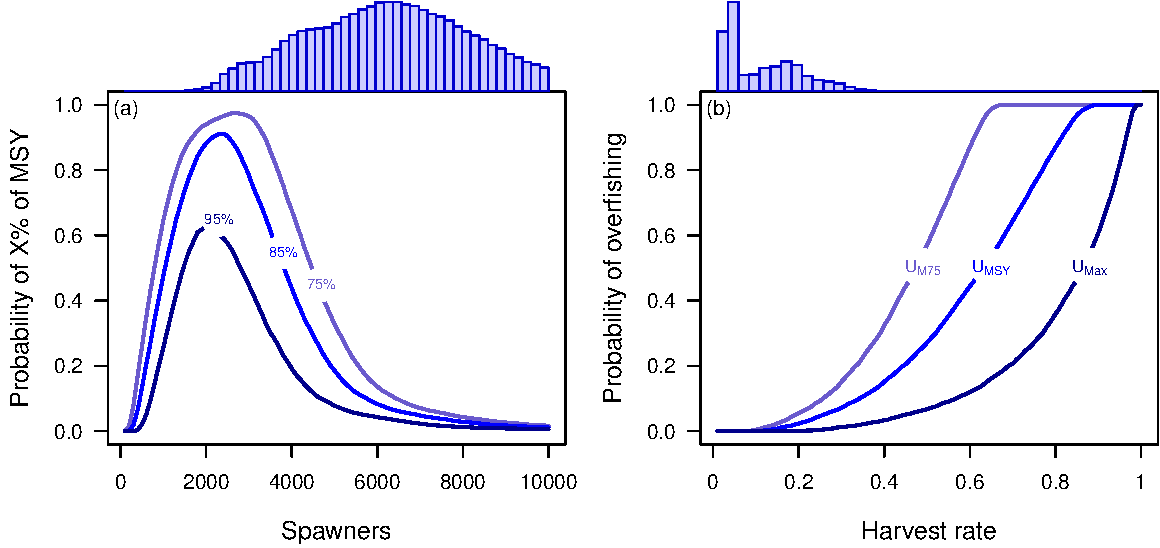
\includegraphics{App_3_Summarize_results_files/figure-latex/fig_6_ref_pts-1} \end{center}

Figure 6. Plots of (a) the probability that a given number of spawners
produces average yields achieving 95\%, 85\%, or 75\% of the estimated
maximum sustainable yield (MSY); and (b) the cumulative probability of
overfishing the population, based on harvest rates equal to those at
75\% of MSY, at MSY, and at the maximum per recruit. The histograms
above (a) and (b) are distributions of the posterior estimates for the
number of spawners and harvest rates, respectively; the histogram in (a)
has been truncated at \(10^4\).


\end{document}
